 \documentclass[10pt, table, dvipsnames,handout]{beamer}
\usetheme[progressbar=frametitle]{metropolis}
\usepackage{appendixnumberbeamer}
\usetikzlibrary{arrows.meta, positioning, quotes}
\usepackage{enumitem}
\usepackage{xcolor}
\usepackage{mathtools}

\usepackage{booktabs}
\usepackage[scale=2]{ccicons}
\usepackage{ dsfont }

\usepackage{pgfplots}
\usepgfplotslibrary{dateplot}

\usepackage{xspace}


\newcommand\hcancel[2][black]{\setbox0=\hbox{$#2$}%
\rlap{\raisebox{.45\ht0}{\textcolor{#1}{\rule{\wd0}{1pt}}}}#2} 

\newcommand{\themename}{\textbf{\textsc{metropolis}}\xspace}
\newcommand{\cb}{\cellcolor{blue!25}}


% Notation:
\newcommand{\cT}{\ensuremath{\mathcal{T}}}
\newcommand{\cD}{\ensuremath{\mathcal{D}}}
\newcommand{\cX}{\ensuremath{\mathcal{X}}}
\newcommand{\cY}{\ensuremath{\mathcal{Y}}}
\newcommand{\cZ}{\ensuremath{\mathcal{Z}}}
\newcommand{\cH}{\ensuremath{\mathcal{H}}}

\newcommand{\bR}{\ensuremath{\mathbb{R}}}
\newcommand{\bN}{\ensuremath{\mathbb{N}}}
\newcommand{\bP}{\ensuremath{\mathbb{P}}}
\newcommand{\bT}{\ensuremath{\mathbb{T}}}
\newcommand{\bL}{\ensuremath{\mathbb{L}}}

\newcommand{\bfX}{\ensuremath{\mathbf{X}}}
\newcommand{\bfY}{\ensuremath{\mathbf{Y}}}


% Tikz seys
\tikzset{cross/.style={cross out, draw, 
         minimum size=2*(#1-\pgflinewidth), 
         inner sep=0pt, outer sep=0pt}}
         
         

\title{Machine Learning I}
\subtitle{Lecture 19: No Free Lunch}
% \date{\today}
\date{}
\author{Nathaniel Bade}
\institute{Northeastern University Department of Mathematics}
% \titlegraphic{\hfill\includegraphics[height=1.5cm]{logo.pdf}}

\begin{document}

\maketitle

\begin{frame}{Table of contents}
  \setbeamertemplate{section in toc}[sections numbered]
  \tableofcontents[hideallsubsections]
\end{frame}





%%%%%%%%%%%%%% Uniform Convergence %%%%%%%%%%%%%% 

\section{Proving Bounds in APAC}

\begin{frame}[fragile]{Proving Bounds in APAC}
\textbf{Goal:} Prove that every finite hypothesis class is APAC learnable. \newline\pause

To work in the APAC framework we need some tools: 

\begin{itemize}
\item[] \textbf{Uniform convergence} - Describes the training sets that lead to small error. 
\item[] \textbf{Hoeffding's Inequality} - Bounds the probability of finding such a training set. 
\end{itemize}


\end{frame}




\begin{frame}[fragile]{$\mathbf{\epsilon}$-Representative Training Sets}
If a hypothesis class is APAC learnable, running $ERM(h)$ on a training set $\mathcal{T}$ will minimize the true error.\newline

It suffices to ensure that the empirical risk $L_\cT(h)$ is a good indicator of the true risk $L_\cD(h)$ for all $h\in \cH$. \pause

A training set $\mathcal{T}$ is called \textbf{$\mathbf{\epsilon}$-representative} (w.r.t. $\cZ$, $\cH$, $\ell$ and $\cD$) if
$$
\forall h\in \mathcal{H},\,\,\, |L_\cT(h) - L_\cD(h)|\leq \epsilon\,,
$$\pause
that is, if empirical risk on $\cT$ is a good indicator of the true risk on $\cZ$. 

\end{frame}




\begin{frame}[fragile]{$\mathbf{\epsilon}$-Representative Training Sets}
\textbf{Lemma:} If a training set is $\epsilon/2$-representative, then any output of $ERM_\cH(\cT)$ (that is any $h_\cT\in \text{argmin}_{h\in\cH}L_\cT(h)$) satisfies 
$$
L_\cD(h_\cT) \leq \min_{h\in \cH}\, L_\cD(h) + \epsilon\,.
$$\pause

\textbf{Proof:} For every $h\in \cH$, 
$$
L_\cD(h_\cT)  \underset{\epsilon-rep}{\leq} L_\cT(h_\cT) + \frac\epsilon2 \pause \underset{ERM}{\leq}  L_\cT(h) + \frac\epsilon2  \pause \underset{\epsilon-rep}{\leq}  L_\cD(h) + \epsilon\,.
$$
\hspace*{\fill}$\Box$

\end{frame}



\begin{frame}[fragile]{Uniform Convergence}
\textbf{Uniform Convergence:} A hypothesis class has the uniform convergence property (w.r.t. $Z$ and $\ell$) if there exists a function $N^{UC}_\cH:(0,1)^2\to\mathbb{N}$ such that for every $\epsilon,\delta \in (0,1)$, if $\cT$ is a training set of size $N\geq N^{UC}_\cH(\epsilon, \delta)$ then, with a probability of at least $1-\delta$ it is $\epsilon$-representative.\newline\pause

\textbf{Corollary:} If a class has the uniform convergence property, then it is APAC learnable by ERM with sample complexity $N^{UC}_\cH$.

\end{frame}




\begin{frame}[fragile]{Hoeffding's Inequality}
We now have a criteria for APAC learnability in terms of the sample sets $\cT$, but we need some tools from probability to estimate expectation values. \newline\pause

\textbf{Hoeffding's Inequality:} Let $\theta_1,\ldots, \theta_N$ be independent random variables with $\bP[a\leq \theta\leq b] = 1$. Define $\theta = \sum \theta_i$. Then for any $\epsilon>0$, 
$$
\bP\left[\, \left|\frac{1}{N} \sum_{i=1}^N(\theta_i - E[\theta]\,)\right|>\epsilon  \,\right]\leq 2\exp\left(-2N\epsilon^2/(b-a)^2\right)\,.
$$
\end{frame}



\begin{frame}[fragile]{Hoeffding's Inequality}
\textbf{Hoeffding's Inequality:} Let $\theta_1,\ldots, \theta_N$ be independent random variables with $\bP[a\leq \theta\leq b] = 1$. Define $\theta = \sum \theta_i$. Then for any $\epsilon>0$, 
$$
\visible<4->{\delta} = \bP\left[\, \left|\frac{1}{N} \sum_{i=1}^N(\theta_i - E[\theta]\,)\right|>\epsilon  \,\right]\leq 2\exp\left(-2N\epsilon^2/(b-a)^2\right)\,.
$$
\rule{\textwidth}{0.4pt}\pause

\textbf{Relation to APAC:} Setting $\theta_i = \ell(h,z_i)$ immediately gives 
$$
L_\cT(h) = \frac{1}{N} \sum_{i=1}^N \ell(h,z_i) =  \frac{1}{N} \sum_{i=1}^N \theta_i\,,\pause
$$ 
and $L_\cD(h) = \frac{1}{N} \sum_{i=1}^N E[\theta_i] = E[\ell(h,z)] = E[\theta]$. \pause So 
$$
\delta = \cD\Big(\,\big\{\mathcal{T}:|L_\cT(h) - L_\cD(h)|>\epsilon\big\}\Big)\,.
$$

\end{frame}





%%%%%%%%%%%%%% Finite Model Spaces are PAC Learnable %%%%%%%%%%%%%% 
\section{Finite Hypothesis Classes are APAC Learnable}


\begin{frame}[fragile]{Finite Hypothesis Classes are APAC Learnable}
We are in a position to prove our first big theorem. The fact that finite hypothesis classes are APAC learnable is an important yardstick in machine learning both as a theoretical comparison and because practically our hypothesis classes aren't infinite.\newline\pause

For example, $\mathcal{H}$ could be the set of predictors that can be implement in $10^{10}$ bits in Python. Our mango example is infinite, but if we discretize it (say by encoding the color and softness parameters as 64 bit floats) it becomes finite. \pause\newline

In fact, any time we discretize the data, the set of all functions $h:\mathcal{X}\to\mathcal{Y}$ be comes finite. However, this doesn't necessarily fix things for us; as we just saw accuracy isn't cheap.
\end{frame}



\begin{frame}[fragile]{Finite Hypothesis Classes are APAC Learnable}
\textbf{Finite Hypothesis Classes are APAC Learnable:}
Let $(\mathcal{Z},\cD,\ell)$ be a domain, distribution and loss function and let $\cH$ be a finite hypothesis class. Fix $\epsilon,\delta\in (0,1)$. \pause 

By uniform convergence, we need to find a sample size $N$ the guarantees (with probability at least $1-\delta$) that if $|\mathcal{T}|>N$, for all $h\in \mathcal{H}$, 
$$
|L_\cT(h) - L_\cD(h)|\leq \epsilon.
$$
\pause 
This is equivalent to showing
$$
\cD^N\Big(\big\{\cT:\exists h\in \mathcal{H}\,,|L_\cT(h)-L_\cD(h)|>\epsilon\big\}\Big)<\delta\,.
$$ 
\end{frame}



\begin{frame}[fragile]{Finite Hypothesis Classes are APAC Learnable}
\textbf{Finite Hypothesis Classes are APAC Learnable:}
Let $(\mathcal{Z},\cD,\ell)$ be a domain, distribution and loss function and let $\cH$ be a finite hypothesis class. Fix $\epsilon,\delta\in (0,1)$. 

By uniform convergence, we need to find a sample size $N$ the guarantees (with probability at least $1-\delta$) that $h\in \mathcal{H}$, 
$$
|L_\cT(h) - L_\cD(h)|\leq \epsilon.
$$
This is equivalent to showing
$$
\cD^N\Big(\,\boxed{\big\{\cT:\exists h\in \mathcal{H}\,,|L_\cT(h)-L_\cD(h)|>\epsilon\big\}}\,\Big)<\delta\,.
$$ 
Lets describe the set of bad training sets. 
\end{frame}




\begin{frame}[fragile]{Finite Hypothesis Classes are APAC Learnable}
The set of bad training sets can be written as the union of the bad sets for each $h$: 
$$
\big\{\cT:\exists h\in \mathcal{H}\,,|L_\cT(h)-L_\cD(h)|>\epsilon\big\} = \bigcup_{h\in\cH} \big\{\cT:|L_\cT(h)-L_\cD(h)|>\epsilon\big\}\,.
$$\pause
We then use the union bound to write
\begin{align*}
\cD^N\Big(\big\{\cT:\exists h\in \mathcal{H}\,,&|L_\cT(h)-L_\cD(h)|>\epsilon\big\}\Big)
\\
&\leq \sum_{h\in\cH}\cD^N\Big(\big\{\cT:\mathcal{H}\,,|L_\cT(h)-L_\cD(h)|>\epsilon\big\}\Big)\,.
\end{align*}
\end{frame}




\begin{frame}[fragile]{Finite Hypothesis Classes are APAC Learnable}
Let $\theta_i = \ell(h,z_i)$. Since $h$ is fixed and $z_i$ are i.i.d., $\theta_i$ are also i.i.d.. As before, $L_\cT(h) = \frac{1}{N}\sum\theta_i$ and $L_\cD(h) = E[\ell(h,z_i)] = \mu$. Finally, for simplicity, lets assume that the range of $\ell$ is $[0,1]$. \pause Hoeffding's inequality gives that for any $h\in \cH$,
\begin{align*}
\cD^N\Big(\big\{\cT:\,|L_\cT(h)-L_\cD(h)|>\epsilon\big\}\Big) 
= \bP\left[\left| \frac{1}{N}\sum_{i=1}^N\theta_i-\mu \right|>\epsilon\right] \leq 2e^{-2N\epsilon^2}\,.
\end{align*}\pause
Summing over the contributions for all $h\in \cH$ yields
\begin{align*}
\cD^N\Big(\big\{\cT:\exists h\in \mathcal{H}\,,|L_\cT(h)-L_\cD(h)|>\epsilon\big\}\Big)&\leq \sum_{h\in\cH}2e^{-2N\epsilon^2}
\\
&=2|\cH|e^{-2N\epsilon^2}\,.
\end{align*}
\end{frame}




\begin{frame}[fragile]{Finite Hypothesis Classes are APAC Learnable}
Therefore, if we choose
\begin{align*}
N\geq \frac{\log(2|\cH|/\delta)}{2\epsilon^2}\,,
\end{align*}
then 
\begin{align*}
\cD^N\Big(\big\{\cT:\exists h\in \mathcal{H}\,,|L_\cT(h)-L_\cD(h)|>\epsilon\big\}\Big)<\delta\,.\,\,\,\Box
\end{align*}
\end{frame}



\begin{frame}[fragile]{Finite Hypothesis Classes are APAC Learnable}
\textbf{Finite Hypothesis Classes are APAC Learnable:}
We have shown that $\mathcal{H}$ enjoys the uniform convergence property with
$$
N_{\cH}^{UC}(\epsilon,\delta)\leq \text{ceil }\left(\frac{\log(2|\cH|/\delta)}{2\epsilon^2}\right)\,.
$$\pause
Therefore, the class is APAC learnable using ERM with sample complexity 
$$
N_{\cH}(\epsilon,\delta)\leq N_{\cH}^{UC}(\epsilon/2,\delta) \leq \text{ceil }\left(\frac{2\log(2|\cH|/\delta)}{\epsilon^2}\right)\,.
$$
\end{frame}



\begin{frame}[fragile]{Discretizing}
As a final note, we can discretize a infinite hypothesis class to get a rough bound on the complexity. \pause For example, each function in the class of interval indicators $I_{[a,b]}$ depends on two real parameters $a,b\in \bR$ which we could represent as, say, 64 bit floats. In general, if we represent $d$ parameters as $b$ bit floats, there are at most
$$
2^{d\times b}
$$
such functions in $\cH$. \pause Applying the bound for finite classes, the sample complexity is at most
$$
N\leq \frac{b\cdot d \log 4+2\log(2/\delta)}{\epsilon^2}\,.
$$
The sample complexity is linear in the number of parameters. 

\end{frame}







\section{No Free Lunch}

\begin{frame}[fragile]{Prior Knowledge}
Overfitting can mislead statistical learning, leading to a large difference between the empirical error and the true error. 

In the last leccture, we saw that if a hypothesis class is PAC/APAC learnable, then with sufficient data we can effectively overcome the problem of over fitting. Precisely, with probability $1-\delta$ the learner returns a classifier with true error within $\epsilon$ of the lowest true error of all classifiers in the hypothesis class. 

For finite hypothesis classes, we showed that the sample complexity was bounded by
$$
N_{\cH}(\epsilon,\delta)\leq \text{ceil }\left(\frac{2\log(2|\cH|/\delta)}{\epsilon^2}\right)\,.
$$
\end{frame}




\begin{frame}[fragile]{Prior Knowledge}
  \begin{minipage}[t][0.5\textheight][t]{\textwidth}
    \begin{overprint}
	  \onslide<1|handout:1> \centering \includegraphics[height=0.5\textheight]{L4HypoRest1.png}
	  \onslide<2|handout:2> \centering \includegraphics[height=0.5\textheight]{L4HypoRest2.png}
	  \onslide<3|handout:3> \centering \includegraphics[height=0.5\textheight]{L4HypoRest3.png}
    \end{overprint}
  \end{minipage}
  \vfill
  \begin{minipage}[t][0.5\textheight][t]{\textwidth}
	However, the choice of how to construct an appropriate hypothesis class seems to require an understanding of the problem. How was the data generated? Can we get a rough idea of the distribution on $\mathcal{X}$? A rough idea of the labeling scheme?
  \end{minipage}


\end{frame}





\begin{frame}[fragile]{Prior Knowledge}
All of the considerations above are known as \textbf{prior knowledge}, and they immediately raise another question: Is prior knowledge necessary? Is there a best algorithm for fitting data whose input is $\cX = \bR^n$, \textit{regardless of the distribution}?\pause

More precisely, a specific \textbf{learning task} is defined by an unknown distribution $\cD$ over $\cX\times \cY$. For a learning task, the goal of the learner is to find a predictor $h$ whose true error is small with respect to $\mathcal{D}$.
\end{frame}




\begin{frame}[fragile]{Prior Knowledge}
For example, classifying $100\times 100$ pixel pictures as cats or dogs has the same sample space $\cX\times\cY = R^{100\times 100}\times \{0,1\}$ as classifying $100\times 100$ pixel MRI scans as containing cancerous cells or not. The only difference between the tasks are the distributions on $\cX\times \cY$.  \pause

Does there exist a universal learner that can account for both cases? Is there an $A$ and an $N$ such that if $A$ receives a training set of $N$ i.i.d. samples it will (probably) return a predictor $h$ with low risk, regardless of $\cD$?\pause

The \textbf{no free lunch theorem} answers that question in the negative: For binary classification, every learner $A$ has a distribution on which is fails.

\end{frame}




\begin{frame}[fragile]{Failure of Learning}
  \begin{minipage}[t][0.5\textheight][t]{\textwidth}
	  \centering \includegraphics[height=0.5\textheight]{L4LinearClass4.png}
  \end{minipage}
  \vfill
  \begin{minipage}[t][0.5\textheight][t]{\textwidth}
For a learner to have ``failed", there must exist an algorithm that can learn the distribution. There are certain distributions on which no learner can do well. \pause

For example, it would not be a failure of the learner to have accuracty $1/2$ for a uniform random binary distribution on which every point had an equal probability of returning either label.  

\end{minipage}
\end{frame}




\begin{frame}[fragile]{Failure of Learning}
  \begin{minipage}[t][0.5\textheight][t]{\textwidth}
    \begin{overprint}
	  \onslide<1|handout:0> \centering \includegraphics[height=0.5\textheight]{L4LinearClass1.png}
	  \onslide<2,3,4|handout:1> \centering \includegraphics[height=0.5\textheight]{L4LinearClass2.png}
    \end{overprint}
  \end{minipage}
  \vfill
  \begin{minipage}[t][0.5\textheight][t]{\textwidth}
Now, a learner might do well given one distribution on $\cX\times \cY$ but fail quite horribly on another. \visible<3->{The challenge becomes cooking up a distribution on which a given learning algorithm fails.}\newline

\visible<4->{
\textbf{Question:} Can you think of a learnable distribution on which the linear classifier fails?
}
\end{minipage}
\end{frame}








\begin{frame}[fragile]{Statement}

\textbf{No Free Lunch Theorem:} Let $A$ be a learning algorithm for the task of binary classification with respect to 0-1 loss. Here, $\cX$ may be arbitrary but $\cY=\{0,1\}$. Let $N\leq |\cX|/2$. Then, there exists a distribution $\mathcal{D}$ over $\cX \times [0,1]$ such that
\begin{enumerate}
\item[1.] There exists $f:\cX\to[0,1]$ with $L_\cD(f) = 0$.
\item[2.] With probability $\delta>1/7$, $L_\cD(A(T))\geq 1/8$. 
\end{enumerate}

\textbf{Comments}: In words, every learner $A$ on $\mathcal{X}\times\mathcal{Y}$ has a learnable task (ie a distribution) on which it fails. \pause The condition $N\leq |\cX|/2$ is technical but intuitive, if a learner has access to all the data we would expect the theorem not to hold. 

\end{frame}






\begin{frame}[fragile]{Ideas in Proof}
The high level idea of the proof is very simple: Imagine I have 2N socks in a drawer, each of which can be one of two colors. I allow you to take a sample of size $N$ out and using any method you want determine the color of the other $N$ socks. How well do you expect to do?

Over the space of all distributions the answer is fairly straight forward: You expect to classify about 1/4 of the socks incorrectly. The half you picked out you'll get correct, as well as half of the remaining, but there is no way you can make a strong inference about the remaining socks if we allow any possible distribution, they simply could be any color. 

The no free lunch theorem formalizes this in the context of more general machine learning problems. 
\end{frame}




\begin{frame}[fragile]{Ideas in Proof}
The no free lunch theorem formalizes this in the context of more general machine learning problems. 

\begin{itemize}
\item We reduce our problem to a problem over discrete distributions.  \pause
\item We then give a concrete description of the space of all deterministic labelings. \pause
\item Finally, we show that the expected error over this space is indeed $1/4$. 
\end{itemize}


\end{frame}








\begin{frame}[fragile]{Ideas in Proof: Discretizing}
  \begin{minipage}[t][0.5\textheight][t]{\textwidth}
	  \centering \includegraphics[height=0.5\textheight]{L4NFLExp1.png}
  \end{minipage}
  \vfill
  \begin{minipage}[t][0.5\textheight][t]{\textwidth}
Lets see why we only need to solve the discrete problem, even if $\mathcal{X}$ is continuous.

Assume that $\mathcal{X}$ is given, as well as a labeling distribution on $\mathcal{X}\times \mathcal{Y}$. For example, in the figure above we have plotted $P(X|Y = 1)$. 

\end{minipage}

\end{frame}


\begin{frame}[fragile]{Ideas in Proof: Discretizing}
  \begin{minipage}[t][0.5\textheight][t]{\textwidth}
	  \centering \includegraphics[height=0.5\textheight]{L4NFLExp1.png}
  \end{minipage}
  \vfill
  \begin{minipage}[t][0.5\textheight][t]{\textwidth}
Given any set of sample points $C\subseteq \cX$, restricting the space of all distributions to those sample points is the same as finding a distribution over the finite set $C$. Practically, this means that in a learning problem the space of all distributions over $\cX\times \cY$ reduces to the space of all distributions over our sample, and possibly a finite number of other points. 
\end{minipage}

\end{frame}



\begin{frame}[fragile]{Ideas in Proof: Discretizing}
  \begin{minipage}[t][0.5\textheight][t]{\textwidth}
	  \centering \includegraphics[height=0.5\textheight]{L4NFLExp2.png}
  \end{minipage}
  \vfill
  \begin{minipage}[t][0.5\textheight][t]{\textwidth}
Given any set of sample points $C\subseteq \cX$, restricting the space of all distributions to those sample points is the same as finding a distribution over the finite set $C$. Practically, this means that in a learning problem the space of all distributions over $\cX\times \cY$ reduces to the space of all distributions over our sample, and possibly a finite number of other points. 
\end{minipage}

\end{frame}




\begin{frame}[fragile]{Ideas in Proof: Discretizing}
  \begin{minipage}[t][0.5\textheight][t]{\textwidth}
	  \centering \includegraphics[height=0.5\textheight]{L4NFLExp3.png}
  \end{minipage}
  \vfill
  \begin{minipage}[t][0.5\textheight][t]{\textwidth}
Given any set of sample points $C\subseteq \cX$, restricting the space of all distributions to those sample points is the same as finding a distribution over the finite set $C$. Practically, this means that in a learning problem the space of all distributions over $\cX\times \cY$ reduces to the space of all distributions over our sample, and possibly a finite number of other points. 
\end{minipage}

\end{frame}





\begin{frame}[fragile]{Ideas in Proof: Space of Deterministic Labelings}
  \begin{minipage}[t][0.4\textheight][t]{\textwidth}
	  	\centering
	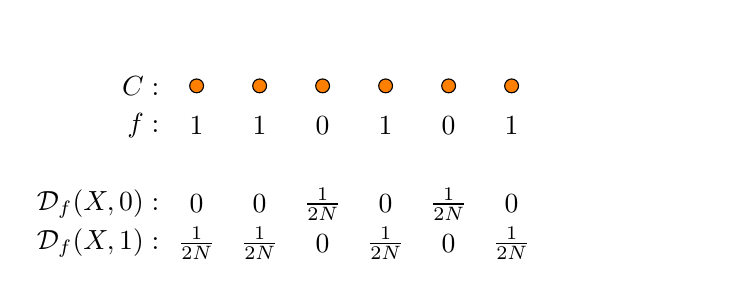
\begin{tikzpicture}[
		sy-/.style = {yshift= -5mm}, 
		sy+/.style = {yshift= 5mm}, 
		yshift=-3.5cm
		]

		
		\node(x1)[circle,draw=black, fill=orange, inner sep=0pt,minimum size=5pt] at (-2,0) {};
		\node(x2)[circle,draw=black, fill=orange, inner sep=0pt,minimum size=5pt] at (-1.2,0) {};
		\node(x3)[circle,draw=black, fill=orange, inner sep=0pt,minimum size=5pt] at (-.4,0) {};
		\node(x4)[circle,draw=black, fill=orange, inner sep=0pt,minimum size=5pt] at (.4,0) {};
		\node(x5)[circle,draw=black, fill=orange, inner sep=0pt,minimum size=5pt] at (1.2,0) {};
		\node(x6)[circle,draw=black, fill=orange, inner sep=0pt,minimum size=5pt] at (2,0) {};

		\node[right,color=Purple,opacity=0] at (x6) {$\hspace{1em}\cT$-sampled};
		\node[right,color=ForestGreen,opacity=0] at ([sy-]x6) {$\hspace{1em}U$-unsampled};
		\node[right,color=ForestGreen,opacity=0] at ([sy+]0,0) {Placeholder};
		
		\node[left] at (x1) {$C:\hspace{1em}$};

		\visible<2->{
		\node[left] at ([sy-]x1) {$f:\hspace{1em}$};	
		\node at ([sy-]x1){1};
		\node at ([sy-]x2){1};
		\node at ([sy-]x3){0};
		\node at ([sy-]x4){1};
		\node at ([sy-]x5){0};
		\node at ([sy-]x6){1};
		}

		\visible<3->{
		\node[left] at ([sy-,sy-,sy-]x1) {$\cD_f(X,0):\hspace{1em}$};	
		\node[left] at ([sy-,sy-,sy-,sy-]x1) {$\cD_f(X,1):\hspace{1em}$};	

		\node at ([sy-,sy-,sy-]x1){0};
		\node at ([sy-,sy-,sy-]x2){0};
		\node at ([sy-,sy-,sy-]x3){$\frac{1}{2N}$};
		\node at ([sy-,sy-,sy-]x4){0};
		\node at ([sy-,sy-,sy-]x5){$\frac{1}{2N}$};
		\node at ([sy-,sy-,sy-]x6){0};

		\node at ([sy-,sy-,sy-,sy-]x1){$\frac{1}{2N}$};
		\node at ([sy-,sy-,sy-,sy-]x2){$\frac{1}{2N}$};
		\node at ([sy-,sy-,sy-,sy-]x3){0};
		\node at ([sy-,sy-,sy-,sy-]x4){$\frac{1}{2N}$};
		\node at ([sy-,sy-,sy-,sy-]x5){0};
		\node at ([sy-,sy-,sy-,sy-]x6){$\frac{1}{2N}$};
		}
	\end{tikzpicture}
  \end{minipage}
  \vfill
  \begin{minipage}[t][0.6\textheight][t]{\textwidth}
We will work over labelings of the discrete set $C\subset \cX$, where $|C| = 2N$. \pause The space of all labelings $\mathbb{L}$ is finite and contains $2^{2N}$ labels $f:C\mapsto \{0,1\}$. \pause

For each labeling $f\in \mathbb{L}$, we define the deterministic distribution, uniform over $C$:
$$
\cD_f((X,Y)) = \begin{cases}
\frac{1}{2N}&\text{if $f(X) = Y$}\,,
\\
0&\text{otherwise}\,.
\end{cases}
$$
This distribution is the nonmixing distribution with labels given by $f$.
\end{minipage}

\end{frame}




\begin{frame}[fragile]{Ideas in Proof: Space of Deterministic Labelings}
  \begin{minipage}[t][0.4\textheight][t]{\textwidth}
	  	\centering
	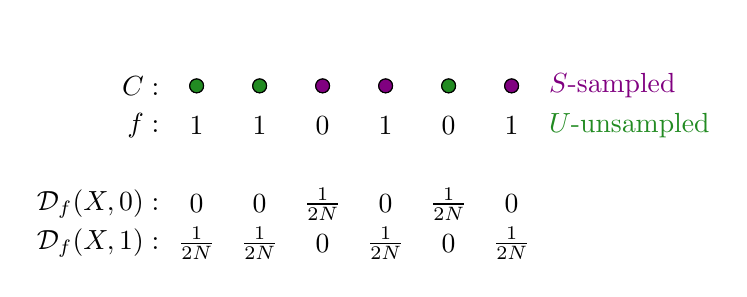
\begin{tikzpicture}[
		sy-/.style = {yshift= -5mm}, 
		sy+/.style = {yshift= 5mm}, 
		]
		\node(x1)[circle,draw=black, fill=orange, inner sep=0pt,minimum size=5pt] at (-2,0) {};
		\node(x2)[circle,draw=black, fill=orange, inner sep=0pt,minimum size=5pt] at (-1.2,0) {};
		\node(x3)[circle,draw=black, fill=orange, inner sep=0pt,minimum size=5pt] at (-.4,0) {};
		\node(x4)[circle,draw=black, fill=orange, inner sep=0pt,minimum size=5pt] at (.4,0) {};
		\node(x5)[circle,draw=black, fill=orange, inner sep=0pt,minimum size=5pt] at (1.2,0) {};
		\node(x6)[circle,draw=black, fill=orange, inner sep=0pt,minimum size=5pt] at (2,0) {};

		\visible<2->{
		\node(x1)[circle,draw=black, fill=ForestGreen, inner sep=0pt,minimum size=5pt] at (-2,0) {};
		\node(x2)[circle,draw=black, fill=ForestGreen, inner sep=0pt,minimum size=5pt] at (-1.2,0) {};
		\node(x3)[circle,draw=black, fill=Purple, inner sep=0pt,minimum size=5pt] at (-.4,0) {};
		\node(x4)[circle,draw=black, fill=Purple, inner sep=0pt,minimum size=5pt] at (.4,0) {};
		\node(x5)[circle,draw=black, fill=ForestGreen, inner sep=0pt,minimum size=5pt] at (1.2,0) {};
		\node(x6)[circle,draw=black, fill=Purple, inner sep=0pt,minimum size=5pt] at (2,0) {};
		
		\node[right,color=Purple] at (x6) {$\hspace{1em}S$-sampled};
		\node[right,color=ForestGreen] at ([sy-]x6) {$\hspace{1em}U$-unsampled};
		\node[right,color=ForestGreen,opacity=0] at ([sy+]0,0) {Placeholder};
		}
		
		\node[left] at (x1) {$C:\hspace{1em}$};


		\node[left] at ([sy-]x1) {$f:\hspace{1em}$};	
		\node at ([sy-]x1){1};
		\node at ([sy-]x2){1};
		\node at ([sy-]x3){0};
		\node at ([sy-]x4){1};
		\node at ([sy-]x5){0};
		\node at ([sy-]x6){1};


		\node[left] at ([sy-,sy-,sy-]x1) {$\cD_f(X,0):\hspace{1em}$};	
		\node[left] at ([sy-,sy-,sy-,sy-]x1) {$\cD_f(X,1):\hspace{1em}$};	

		\node at ([sy-,sy-,sy-]x1){0};
		\node at ([sy-,sy-,sy-]x2){0};
		\node at ([sy-,sy-,sy-]x3){$\frac{1}{2N}$};
		\node at ([sy-,sy-,sy-]x4){0};
		\node at ([sy-,sy-,sy-]x5){$\frac{1}{2N}$};
		\node at ([sy-,sy-,sy-]x6){0};

		\node at ([sy-,sy-,sy-,sy-]x1){$\frac{1}{2N}$};
		\node at ([sy-,sy-,sy-,sy-]x2){$\frac{1}{2N}$};
		\node at ([sy-,sy-,sy-,sy-]x3){0};
		\node at ([sy-,sy-,sy-,sy-]x4){$\frac{1}{2N}$};
		\node at ([sy-,sy-,sy-,sy-]x5){0};
		\node at ([sy-,sy-,sy-,sy-]x6){$\frac{1}{2N}$};

	\end{tikzpicture}
  \end{minipage}
  \vfill
  \begin{minipage}[t][0.6\textheight][t]{\textwidth}
Let $\mathbb{T}$ be the set of all size $N$ samples of the $C$. The cardinality of this set is $|\mathbb{T}| = (2N)^N$, and points may be sampled more than once. For any sampled set $S\in \bT$, let $U = C-S$ be the unsampled points.

\end{minipage}

\end{frame}


\begin{frame}[fragile]{Ideas in Proof: Space of Deterministic Labelings}
  \begin{minipage}[t][0.4\textheight][t]{\textwidth}
	  	\centering
	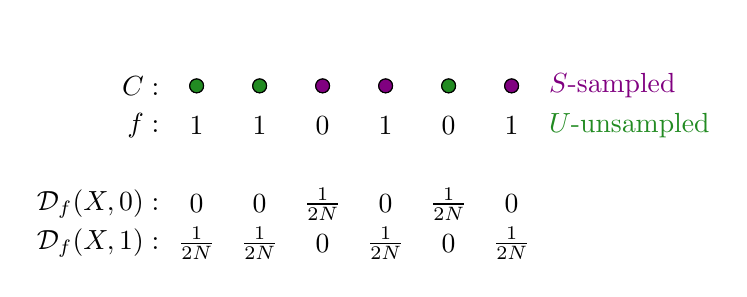
\begin{tikzpicture}[
		sy-/.style = {yshift= -5mm}, 
		sy+/.style = {yshift= 5mm}, 
		]
		\node(x1)[circle,draw=black, fill=orange, inner sep=0pt,minimum size=5pt] at (-2,0) {};
		\node(x2)[circle,draw=black, fill=orange, inner sep=0pt,minimum size=5pt] at (-1.2,0) {};
		\node(x3)[circle,draw=black, fill=orange, inner sep=0pt,minimum size=5pt] at (-.4,0) {};
		\node(x4)[circle,draw=black, fill=orange, inner sep=0pt,minimum size=5pt] at (.4,0) {};
		\node(x5)[circle,draw=black, fill=orange, inner sep=0pt,minimum size=5pt] at (1.2,0) {};
		\node(x6)[circle,draw=black, fill=orange, inner sep=0pt,minimum size=5pt] at (2,0) {};

		\visible<2->{
		\node(x1)[circle,draw=black, fill=ForestGreen, inner sep=0pt,minimum size=5pt] at (-2,0) {};
		\node(x2)[circle,draw=black, fill=ForestGreen, inner sep=0pt,minimum size=5pt] at (-1.2,0) {};
		\node(x3)[circle,draw=black, fill=Purple, inner sep=0pt,minimum size=5pt] at (-.4,0) {};
		\node(x4)[circle,draw=black, fill=Purple, inner sep=0pt,minimum size=5pt] at (.4,0) {};
		\node(x5)[circle,draw=black, fill=ForestGreen, inner sep=0pt,minimum size=5pt] at (1.2,0) {};
		\node(x6)[circle,draw=black, fill=Purple, inner sep=0pt,minimum size=5pt] at (2,0) {};
		
		\node[right,color=Purple] at (x6) {$\hspace{1em}S$-sampled};
		\node[right,color=ForestGreen] at ([sy-]x6) {$\hspace{1em}U$-unsampled};
		\node[right,color=ForestGreen,opacity=0] at ([sy+]0,0) {Placeholder};
		}
		
		\node[left] at (x1) {$C:\hspace{1em}$};


		\node[left] at ([sy-]x1) {$f:\hspace{1em}$};	
		\node at ([sy-]x1){1};
		\node at ([sy-]x2){1};
		\node at ([sy-]x3){0};
		\node at ([sy-]x4){1};
		\node at ([sy-]x5){0};
		\node at ([sy-]x6){1};


		\node[left] at ([sy-,sy-,sy-]x1) {$\cD_f(X,0):\hspace{1em}$};	
		\node[left] at ([sy-,sy-,sy-,sy-]x1) {$\cD_f(X,1):\hspace{1em}$};	

		\node at ([sy-,sy-,sy-]x1){0};
		\node at ([sy-,sy-,sy-]x2){0};
		\node at ([sy-,sy-,sy-]x3){$\frac{1}{2N}$};
		\node at ([sy-,sy-,sy-]x4){0};
		\node at ([sy-,sy-,sy-]x5){$\frac{1}{2N}$};
		\node at ([sy-,sy-,sy-]x6){0};

		\node at ([sy-,sy-,sy-,sy-]x1){$\frac{1}{2N}$};
		\node at ([sy-,sy-,sy-,sy-]x2){$\frac{1}{2N}$};
		\node at ([sy-,sy-,sy-,sy-]x3){0};
		\node at ([sy-,sy-,sy-,sy-]x4){$\frac{1}{2N}$};
		\node at ([sy-,sy-,sy-,sy-]x5){0};
		\node at ([sy-,sy-,sy-,sy-]x6){$\frac{1}{2N}$};

	\end{tikzpicture}
  \end{minipage}
  \vfill
  \begin{minipage}[t][0.6\textheight][t]{\textwidth}
Effectively what we have done is a Cartesian decomposition of the space of training set with arbitrary labels into two pieces: The space of all labels $\bL$ and the space of all sample sets $\bT$.\pause\, A training set is then denoted 
$$
S_f = \{(x,f(x))\,:\, x\in S\}\,.
$$\pause
The set $\bL\times \bT$ is the set of all training sets with any labeling. 

\end{minipage}

\end{frame}






\begin{frame}[fragile]{Ideas in Proof: Space of Deterministic Labelings}
  \begin{minipage}[t][0.4\textheight][t]{\textwidth}
	  	\centering
	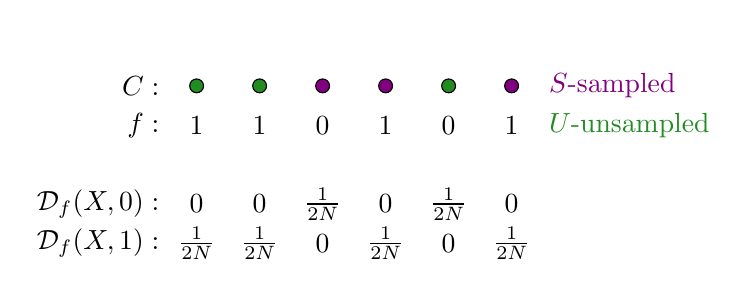
\begin{tikzpicture}[
		sy-/.style = {yshift= -5mm}, 
		sy+/.style = {yshift= 5mm}, 
		]

		\node(x1)[circle,draw=black, fill=ForestGreen, inner sep=0pt,minimum size=5pt] at (-2,0) {};
		\node(x2)[circle,draw=black, fill=ForestGreen, inner sep=0pt,minimum size=5pt] at (-1.2,0) {};
		\node(x3)[circle,draw=black, fill=Purple, inner sep=0pt,minimum size=5pt] at (-.4,0) {};
		\node(x4)[circle,draw=black, fill=Purple, inner sep=0pt,minimum size=5pt] at (.4,0) {};
		\node(x5)[circle,draw=black, fill=ForestGreen, inner sep=0pt,minimum size=5pt] at (1.2,0) {};
		\node(x6)[circle,draw=black, fill=Purple, inner sep=0pt,minimum size=5pt] at (2,0) {};
		
		\node[right,color=Purple] at (x6) {$\hspace{1em}S$-sampled};
		\node[right,color=ForestGreen] at ([sy-]x6) {$\hspace{1em}U$-unsampled};
		\node[right,color=ForestGreen,opacity=0] at ([sy+]0,0) {Placeholder};
		
		\node[left] at (x1) {$C:\hspace{1em}$};


		\node[left] at ([sy-]x1) {$f:\hspace{1em}$};	
		\node at ([sy-]x1){1};
		\node at ([sy-]x2){1};
		\node at ([sy-]x3){0};
		\node at ([sy-]x4){1};
		\node at ([sy-]x5){0};
		\node at ([sy-]x6){1};


		\node[left] at ([sy-,sy-,sy-]x1) {$\cD_f(X,0):\hspace{1em}$};	
		\node[left] at ([sy-,sy-,sy-,sy-]x1) {$\cD_f(X,1):\hspace{1em}$};	

		\node at ([sy-,sy-,sy-]x1){0};
		\node at ([sy-,sy-,sy-]x2){0};
		\node at ([sy-,sy-,sy-]x3){$\frac{1}{2N}$};
		\node at ([sy-,sy-,sy-]x4){0};
		\node at ([sy-,sy-,sy-]x5){$\frac{1}{2N}$};
		\node at ([sy-,sy-,sy-]x6){0};

		\node at ([sy-,sy-,sy-,sy-]x1){$\frac{1}{2N}$};
		\node at ([sy-,sy-,sy-,sy-]x2){$\frac{1}{2N}$};
		\node at ([sy-,sy-,sy-,sy-]x3){0};
		\node at ([sy-,sy-,sy-,sy-]x4){$\frac{1}{2N}$};
		\node at ([sy-,sy-,sy-,sy-]x5){0};
		\node at ([sy-,sy-,sy-,sy-]x6){$\frac{1}{2N}$};

	\end{tikzpicture}
  \end{minipage}
  \vfill
  \begin{minipage}[t][0.6\textheight][t]{\textwidth}

\textbf{Idea:} Let $A(S_f)$ denote the classifier returned by the training set 
$$
S_f = \{(x,f(x))\,:\, x\in S\}\,.
$$\pause 
We will show that
$$
\max_{f\in \mathbb{L}} E_{S}\big[ L_{D_f}(A(S_f)) \big] \geq \frac14\,.
$$\pause

That is, we will show that the maximum (over all labelings) of the expected error (for the classifier returned by $A$ trained on $S_f$) is bounded from below. 


\end{minipage}

\end{frame}





\begin{frame}[fragile]{Ideas in Proof: Space of Deterministic Labelings}
  \begin{minipage}[t][0.4\textheight][t]{\textwidth}
	  	\centering
	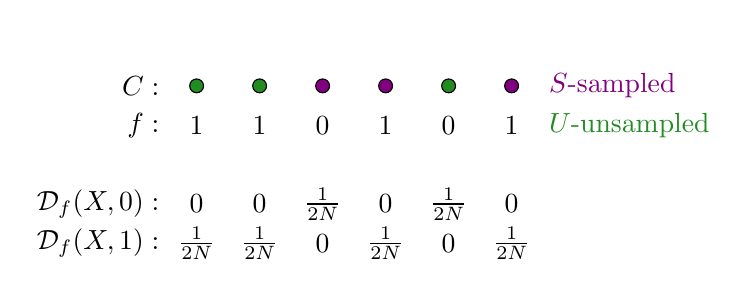
\begin{tikzpicture}[
		sy-/.style = {yshift= -5mm}, 
		sy+/.style = {yshift= 5mm}, 
		]

		\node(x1)[circle,draw=black, fill=ForestGreen, inner sep=0pt,minimum size=5pt] at (-2,0) {};
		\node(x2)[circle,draw=black, fill=ForestGreen, inner sep=0pt,minimum size=5pt] at (-1.2,0) {};
		\node(x3)[circle,draw=black, fill=Purple, inner sep=0pt,minimum size=5pt] at (-.4,0) {};
		\node(x4)[circle,draw=black, fill=Purple, inner sep=0pt,minimum size=5pt] at (.4,0) {};
		\node(x5)[circle,draw=black, fill=ForestGreen, inner sep=0pt,minimum size=5pt] at (1.2,0) {};
		\node(x6)[circle,draw=black, fill=Purple, inner sep=0pt,minimum size=5pt] at (2,0) {};
		
		\node[right,color=Purple] at (x6) {$\hspace{1em}S$-sampled};
		\node[right,color=ForestGreen] at ([sy-]x6) {$\hspace{1em}U$-unsampled};
		\node[right,color=ForestGreen,opacity=0] at ([sy+]0,0) {Placeholder};
		
		
		\node[left] at (x1) {$C:\hspace{1em}$};


		\node[left] at ([sy-]x1) {$f:\hspace{1em}$};	
		\node at ([sy-]x1){1};
		\node at ([sy-]x2){1};
		\node at ([sy-]x3){0};
		\node at ([sy-]x4){1};
		\node at ([sy-]x5){0};
		\node at ([sy-]x6){1};


		\node[left] at ([sy-,sy-,sy-]x1) {$\cD_f(X,0):\hspace{1em}$};	
		\node[left] at ([sy-,sy-,sy-,sy-]x1) {$\cD_f(X,1):\hspace{1em}$};	

		\node at ([sy-,sy-,sy-]x1){0};
		\node at ([sy-,sy-,sy-]x2){0};
		\node at ([sy-,sy-,sy-]x3){$\frac{1}{2N}$};
		\node at ([sy-,sy-,sy-]x4){0};
		\node at ([sy-,sy-,sy-]x5){$\frac{1}{2N}$};
		\node at ([sy-,sy-,sy-]x6){0};

		\node at ([sy-,sy-,sy-,sy-]x1){$\frac{1}{2N}$};
		\node at ([sy-,sy-,sy-,sy-]x2){$\frac{1}{2N}$};
		\node at ([sy-,sy-,sy-,sy-]x3){0};
		\node at ([sy-,sy-,sy-,sy-]x4){$\frac{1}{2N}$};
		\node at ([sy-,sy-,sy-,sy-]x5){0};
		\node at ([sy-,sy-,sy-,sy-]x6){$\frac{1}{2N}$};

	\end{tikzpicture}
  \end{minipage}
  \vfill
  \begin{minipage}[t][0.6\textheight][t]{\textwidth}
This 1/4 bound has a simple interpretation: Since we may draw the same point more than once, $|S|\leq 2N$ and $|U|\geq 2N$. That means that any algorithm isn't going to know how to label the (possibly more than) $\frac12$ of the data in $U$. \pause 

Furthermore, we would imagine that on average the algorithm will mislabel approximately 50\% of the labels. So no matter what the algorithm is it should mislabel around 1/4 of the points. 


\end{minipage}

\end{frame}



\begin{frame}[fragile]{Ideas in Proof: Min/Max Swap}
 We will use the following trick one and a half times: 

Let $\cD$ be a joint distribution on $\mathcal{X}\times\cY$ and let $g:\cX\times \cY\to \bR_+$ be a positive function.  We can bound the maximum of the expectation value with respect to one variable by the minimum expectation value with respect to the other:\pause
\begin{align*}
\max_{X} E_{Y}\big[ g(X,Y) \big] &\geq E_{X} E_{Y}\big[ g(X,Y) \big]   
\\
&\geq E_{Y} E_{X}\big[ g(X,Y) \big]   && \text{by Fubini's Theorem}
\\
&\geq 
\min_{Y} E_{X}\big[ g(X,Y) \big] 
\end{align*}\pause
This might seem very trivial, but we will use it swap between expectations over the labels $\mathbb{L}$ and over the sample sets $\mathbb{T}$. 
\end{frame}

\section{Proof of No Free Lunch Theorem}


\begin{frame}[fragile]{Min/Max Swap}
  \begin{minipage}[t][0.4\textheight][t]{\textwidth}
	  	\centering
	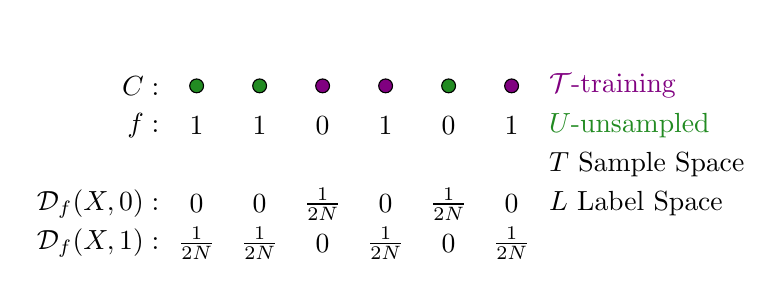
\begin{tikzpicture}[
		sy-/.style = {yshift= -5mm}, 
		sy+/.style = {yshift= 5mm}, 
		]

		\node(x1)[circle,draw=black, fill=ForestGreen, inner sep=0pt,minimum size=5pt] at (-2,0) {};
		\node(x2)[circle,draw=black, fill=ForestGreen, inner sep=0pt,minimum size=5pt] at (-1.2,0) {};
		\node(x3)[circle,draw=black, fill=Purple, inner sep=0pt,minimum size=5pt] at (-.4,0) {};
		\node(x4)[circle,draw=black, fill=Purple, inner sep=0pt,minimum size=5pt] at (.4,0) {};
		\node(x5)[circle,draw=black, fill=ForestGreen, inner sep=0pt,minimum size=5pt] at (1.2,0) {};
		\node(x6)[circle,draw=black, fill=Purple, inner sep=0pt,minimum size=5pt] at (2,0) {};
		
		\node[right,color=Purple] at (x6) {$\hspace{1em}\cT$-training};
		\node[right,color=ForestGreen] at ([sy-]x6) {$\hspace{1em}U$-unsampled};

		\node[right] at ([sy-,sy-]x6) {$\hspace{1em}\mathbb{T}$ Sample Space};
		\node[right] at ([sy-,sy-,sy-]x6) {$\hspace{1em}\mathbb{L}$ Label Space};

		\node[right,color=ForestGreen,opacity=0] at ([sy+]0,0) {Placeholder};
		
		
		\node[left] at (x1) {$C:\hspace{1em}$};


		\node[left] at ([sy-]x1) {$f:\hspace{1em}$};	
		\node at ([sy-]x1){1};
		\node at ([sy-]x2){1};
		\node at ([sy-]x3){0};
		\node at ([sy-]x4){1};
		\node at ([sy-]x5){0};
		\node at ([sy-]x6){1};


		\node[left] at ([sy-,sy-,sy-]x1) {$\cD_f(X,0):\hspace{1em}$};	
		\node[left] at ([sy-,sy-,sy-,sy-]x1) {$\cD_f(X,1):\hspace{1em}$};	

		\node at ([sy-,sy-,sy-]x1){0};
		\node at ([sy-,sy-,sy-]x2){0};
		\node at ([sy-,sy-,sy-]x3){$\frac{1}{2N}$};
		\node at ([sy-,sy-,sy-]x4){0};
		\node at ([sy-,sy-,sy-]x5){$\frac{1}{2N}$};
		\node at ([sy-,sy-,sy-]x6){0};

		\node at ([sy-,sy-,sy-,sy-]x1){$\frac{1}{2N}$};
		\node at ([sy-,sy-,sy-,sy-]x2){$\frac{1}{2N}$};
		\node at ([sy-,sy-,sy-,sy-]x3){0};
		\node at ([sy-,sy-,sy-,sy-]x4){$\frac{1}{2N}$};
		\node at ([sy-,sy-,sy-,sy-]x5){0};
		\node at ([sy-,sy-,sy-,sy-]x6){$\frac{1}{2N}$};

	\end{tikzpicture}
  \end{minipage}
  \vfill
  \begin{minipage}[t][0.6\textheight][t]{\textwidth}
\textbf{Proof of NFL:} Let $C$, $\mathbb{T}$ and $\mathbb{L}$ be as above. We can use the max/min swap to write
$$
\max_{f\in \mathbb{L}} E_{S}\big[ L_{D_f}(A(S_f)) \big] \geq \min_{S\in\mathbb{T}} E_{f\in\mathbb{L}}\big[ L_{D_f}(A(S_f)) \big] \,.
$$
We will now attempt to bound $ L_{D_f}(A(S_f))$.

\end{minipage}
\end{frame}






\begin{frame}[fragile]{Min/Max Swap}
  \begin{minipage}[t][0.4\textheight][t]{\textwidth}
	  	\centering
	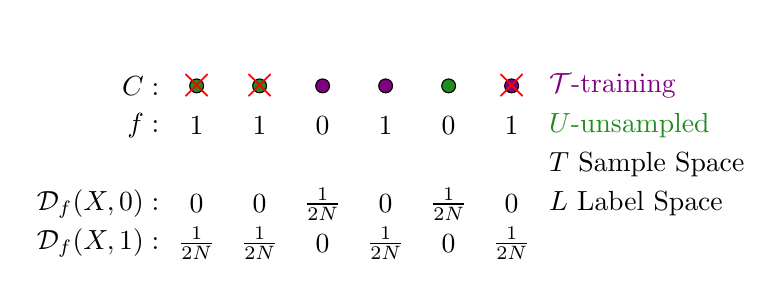
\begin{tikzpicture}[
		sy-/.style = {yshift= -5mm}, 
		sy+/.style = {yshift= 5mm}, 
		]

		\node(x1)[circle,draw=black, fill=ForestGreen, inner sep=0pt,minimum size=5pt] at (-2,0) {};
		\node(x2)[circle,draw=black, fill=ForestGreen, inner sep=0pt,minimum size=5pt] at (-1.2,0) {};
		\node(x3)[circle,draw=black, fill=Purple, inner sep=0pt,minimum size=5pt] at (-.4,0) {};
		\node(x4)[circle,draw=black, fill=Purple, inner sep=0pt,minimum size=5pt] at (.4,0) {};
		\node(x5)[circle,draw=black, fill=ForestGreen, inner sep=0pt,minimum size=5pt] at (1.2,0) {};
		\node(x6)[circle,draw=black, fill=Purple, inner sep=0pt,minimum size=5pt] at (2,0) {};
		
		\visible<2->{
		\node [color=red] at (x6){\LARGE $\times$};
		\node [color=red] at (x1){\LARGE $\times$};
		\node [color=red] at (x2){\LARGE $\times$};
		}
		
		\node[right,color=Purple] at (x6) {$\hspace{1em}\cT$-training};
		\node[right,color=ForestGreen] at ([sy-]x6) {$\hspace{1em}U$-unsampled};

		\node[right] at ([sy-,sy-]x6) {$\hspace{1em}\mathbb{T}$ Sample Space};
		\node[right] at ([sy-,sy-,sy-]x6) {$\hspace{1em}\mathbb{L}$ Label Space};

		\node[right,color=ForestGreen,opacity=0] at ([sy+]0,0) {Placeholder};
		
		
		\node[left] at (x1) {$C:\hspace{1em}$};


		\node[left] at ([sy-]x1) {$f:\hspace{1em}$};	
		\node at ([sy-]x1){1};
		\node at ([sy-]x2){1};
		\node at ([sy-]x3){0};
		\node at ([sy-]x4){1};
		\node at ([sy-]x5){0};
		\node at ([sy-]x6){1};


		\node[left] at ([sy-,sy-,sy-]x1) {$\cD_f(X,0):\hspace{1em}$};	
		\node[left] at ([sy-,sy-,sy-,sy-]x1) {$\cD_f(X,1):\hspace{1em}$};	

		\node at ([sy-,sy-,sy-]x1){0};
		\node at ([sy-,sy-,sy-]x2){0};
		\node at ([sy-,sy-,sy-]x3){$\frac{1}{2N}$};
		\node at ([sy-,sy-,sy-]x4){0};
		\node at ([sy-,sy-,sy-]x5){$\frac{1}{2N}$};
		\node at ([sy-,sy-,sy-]x6){0};

		\node at ([sy-,sy-,sy-,sy-]x1){$\frac{1}{2N}$};
		\node at ([sy-,sy-,sy-,sy-]x2){$\frac{1}{2N}$};
		\node at ([sy-,sy-,sy-,sy-]x3){0};
		\node at ([sy-,sy-,sy-,sy-]x4){$\frac{1}{2N}$};
		\node at ([sy-,sy-,sy-,sy-]x5){0};
		\node at ([sy-,sy-,sy-,sy-]x6){$\frac{1}{2N}$};

	\end{tikzpicture}
  \end{minipage}
  \vfill
  \begin{minipage}[t][0.6\textheight][t]{\textwidth}
For fixed sample $S$, 
$$
L_{D_f}(A(S_f)) = \frac{1}{2N} \sum_{x\in C} 1_{f(x)\neq A(S_f)[x]}
$$
is the number of incorrect predictions divided by $2N$. \pause \pause We expect the error on the sampled set to be low, so we bound by the error on $U$
$$
L_{D_f}(A(S_f)) \geq \frac{1}{2N} \sum_{x\in U} 1_{f(x)\neq A(S_f)[x]}\pause \geq \frac{1}{2|U|} \sum_{x\in U} 1_{f(x)\neq A(S_f)[x]}.
$$

\end{minipage}
\end{frame}






\begin{frame}[fragile]{Min/Max Swap}
Writing then
$$
L_{D_f}(A(Sf)) \geq \frac{1}{2}E_{x\in U}\big[\,  1_{f(x)\neq A(S_f)[x]} \,\big]\,,\pause
$$
we can use the fact the min is at most the expectation value to write
\begin{align*}
 E_{f\in \bL}\big[\,  L_{\cD_f}(A(S_f))\,\big] &\geq  \frac12 E_{f\in \bL} E_{x\in U}\big[\,  1_{f(x)\neq A(S_f)[x]} \,\big]
\\
&\geq  \frac12 \min_{x\in U} E_{f\in \bL}\big[\,  1_{f(x)\neq A(S_f)[x]} \,\big]\,.
\end{align*}\pause
So for a fixed $S$, the average error (over all labelings) is bounded by the 1/2 the average error over the worst element in the unsampled set. 

\end{frame}



\begin{frame}[fragile]{Min/Max Swap}
For every function $f\in \mathbb{L}$, there is a function $f'\in \mathbb{L}$ such that $f$ and $f'$ agree on the sample set $f|_S = f'|_S$, but assign opposite labels to the unsampled set, $f(x)\neq f'(x)$, $\forall x\in U$. \pause For every such a pair
$$
1_{f(x)\neq A(S_f)[x]} + 1_{f'(x)\neq A(S_f)[x]} = 1\,,\,\,\forall x\in U\,.\pause
$$
But then 
$$
E_{f\in \bL}\big[\,  1_{f(x)\neq A(S_f)[x]} \,\big] = \frac{1}{|\mathbb{L}|}\sum_{f\in\mathbb{L}} 1_{f(x)\neq A(S_f)[x]}  = \frac{1}{2}\,.\pause
$$
Lets put it all together.
\end{frame}




\begin{frame}[fragile]{Min/Max Swap}
Lets put it all together.
\begin{align*}
\action<+->{\max_{f\in \mathbb{L}} E_{S}\big[ L_{D_f}(A(S_f)) \big] &\geq \min_{S\in\mathbb{T}} E_{f\in\mathbb{L}}\big[ L_{D_f}(A(S_f)) \big]}
\\
\action<+->{&\geq  
 \min_{S\in\mathbb{T}}
\min_{x\in U}\,\frac12\, E_{f\in \bL}\big[\,  1_{f(x)\neq A(S_f)[x]} \,\big]}
\\
\action<+->{&\geq  
 \min_{S\in\mathbb{T}}
\min_{x\in U}\,\frac12\cdot \frac 12}
\\
\action<+->{&=\frac14\,.}
\end{align*}
\action<+->{We have shown that there is always a labeling on which the risk of an algorithm $A$ is bounded from below. The final step is to show that this result isn't rare.}
\end{frame}




\begin{frame}[fragile]{Min/Max Swap}
  \begin{minipage}[t][0.4\textheight][t]{\textwidth}
	  	\centering
	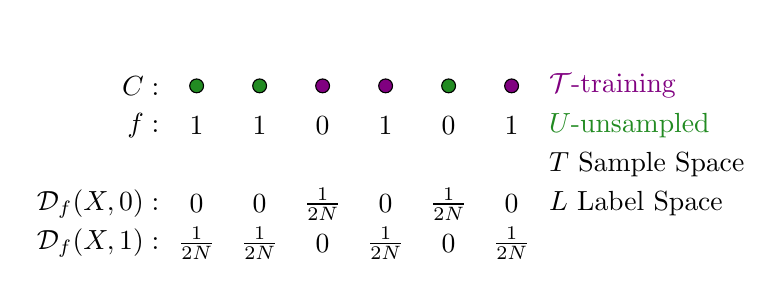
\begin{tikzpicture}[
		sy-/.style = {yshift= -5mm}, 
		sy+/.style = {yshift= 5mm}, 
		]

		\node(x1)[circle,draw=black, fill=ForestGreen, inner sep=0pt,minimum size=5pt] at (-2,0) {};
		\node(x2)[circle,draw=black, fill=ForestGreen, inner sep=0pt,minimum size=5pt] at (-1.2,0) {};
		\node(x3)[circle,draw=black, fill=Purple, inner sep=0pt,minimum size=5pt] at (-.4,0) {};
		\node(x4)[circle,draw=black, fill=Purple, inner sep=0pt,minimum size=5pt] at (.4,0) {};
		\node(x5)[circle,draw=black, fill=ForestGreen, inner sep=0pt,minimum size=5pt] at (1.2,0) {};
		\node(x6)[circle,draw=black, fill=Purple, inner sep=0pt,minimum size=5pt] at (2,0) {};
		
		\node[right,color=Purple] at (x6) {$\hspace{1em}\cT$-training};
		\node[right,color=ForestGreen] at ([sy-]x6) {$\hspace{1em}U$-unsampled};

		\node[right] at ([sy-,sy-]x6) {$\hspace{1em}\mathbb{T}$ Sample Space};
		\node[right] at ([sy-,sy-,sy-]x6) {$\hspace{1em}\mathbb{L}$ Label Space};

		\node[right,color=ForestGreen,opacity=0] at ([sy+]0,0) {Placeholder};
		
		
		\node[left] at (x1) {$C:\hspace{1em}$};


		\node[left] at ([sy-]x1) {$f:\hspace{1em}$};	
		\node at ([sy-]x1){1};
		\node at ([sy-]x2){1};
		\node at ([sy-]x3){0};
		\node at ([sy-]x4){1};
		\node at ([sy-]x5){0};
		\node at ([sy-]x6){1};


		\node[left] at ([sy-,sy-,sy-]x1) {$\cD_f(X,0):\hspace{1em}$};	
		\node[left] at ([sy-,sy-,sy-,sy-]x1) {$\cD_f(X,1):\hspace{1em}$};	

		\node at ([sy-,sy-,sy-]x1){0};
		\node at ([sy-,sy-,sy-]x2){0};
		\node at ([sy-,sy-,sy-]x3){$\frac{1}{2N}$};
		\node at ([sy-,sy-,sy-]x4){0};
		\node at ([sy-,sy-,sy-]x5){$\frac{1}{2N}$};
		\node at ([sy-,sy-,sy-]x6){0};

		\node at ([sy-,sy-,sy-,sy-]x1){$\frac{1}{2N}$};
		\node at ([sy-,sy-,sy-,sy-]x2){$\frac{1}{2N}$};
		\node at ([sy-,sy-,sy-,sy-]x3){0};
		\node at ([sy-,sy-,sy-,sy-]x4){$\frac{1}{2N}$};
		\node at ([sy-,sy-,sy-,sy-]x5){0};
		\node at ([sy-,sy-,sy-,sy-]x6){$\frac{1}{2N}$};

	\end{tikzpicture}
  \end{minipage}
  \vfill
  \begin{minipage}[t][0.6\textheight][t]{\textwidth}
\textbf{Exercise:} Use Markov's Inequality to show that 
$$
\max_{f\in \mathbb{L}} E_{S}\big[ L_{D_f}(A(S_f)) \big] \geq \frac14
$$
implies
$$
\bP\big[\, L_{\cD}(A(S))\geq 1/8 \,\big]\geq 1/7\,.
$$
This final step completes the proof. \pause

\textbf{Question:} What sort of distribution must k-NN fail on?
\end{minipage}
\end{frame}





\section{The Bias-Complexity Tradeoff}
\begin{frame}[fragile]{Avoiding Underfitting}
The no free lunch theorem isn't the end of machine learning, it simply asserts that there is no universally best learner for every task. If fact, it implies that we should use any prior knowledge to avoid learners that perform poorly on a distribution. Such prior knowledge can be expressed by restricting the hypothesis class. \pause

But how do we choose this class? On one hand, we want a class that contains a classifier that will return the minimum error. On the other hand, the class of all functions is clearly not learnable so we cant just choose the richest class. 
\end{frame}



\begin{frame}[fragile]{Bias and Complexity}
To begin to address the question, we decompose the total error
$$
L_\cD(h_\cT) = \underbrace{\min_{h\in \cH}\,L_\cD(h)}_{\epsilon_{app}}
+
\underbrace{\big(L_\cD(h_\cT) - \min_{h\in \cH}\,L_\cD(h)\big)}_{\epsilon_{est}}
$$\pause
into
\begin{itemize}
\item[] \textbf{Approximation Error:} The minimum risk achievable within a class. This term is also known as the \textbf{inductive bias}.
\item[] \textbf{Estimation Error:} The difference between the minimum achievable risk and the ERM error. This is the term to be minimized in APAC.
\end{itemize}\pause
Again: \textbf{APAC learning bounds estimation error.} It fundamentally says nothing about approximation error. 
\end{frame}




\begin{frame}[fragile]{Estimation Error}
We derived an expression for the estimation error of a finite hypothesis class $\cH$. We found, 
$$
\epsilon_{est} = L_\cD(h_\cT) - \min_{h\in \cH}\,L_\cD(h) \geq \left(\frac{\log(2|\cH|/\delta)}{2N}\right)^{\frac12}
\,.
$$\pause
For fixed $\delta$, if the training size $N$ decreases or $|\cH|$ increases (exponentially), the \textbf{estimation error} increases. This justifies thinking of $\epsilon_{est}$ as a measure of relative complexity.
\end{frame}




\begin{frame}[fragile]{Bias and Complexity}
The decomposition
$$
L_\cD(h_\cT) = \underbrace{\min_{h\in \cH}\,L_\cD(h)}_{\epsilon_{app}}
+
\underbrace{\big(L_\cD(h_\cT) - \min_{h\in \cH}\,L_\cD(h)\big)}_{\epsilon_{est}}
$$
is known as the \textbf{bias-complexity trade off}. It states that within a hypothesis class we can trade bias for complexity, but we cannot minimize both. \newline \pause

Note that this decomposition is quite general: it holds regardless of the loss function, the hypothesis class or the learning algorithm. In the rest of this lecture, we will derive more specific results by analyzing the decomposition for our test hypothesis classes, the linear predictors and $k$ nearest neighbors.

\end{frame}



\section{The Bias-Variance Tradeoff: Bias-Complexity for RSS}

\begin{frame}[fragile]{Estimation Error}
There is more we can say if we restrict ourselves to a specific loss function and distribution. Assume for the moment that there is a true labeling function $f:\cX\to\cY$. \pause Consider the pointwise \textbf{mean squared error} of a predictor $h_\cT$ on some $x_0\in \cX$. 
\begin{align*}
MSE(x_0) &= E_\cT[f(x_0)-h_\cT(x_0)]^2
\end{align*}\pause
Define $y_0^\cH:=E_\cT[h_\cT(x_0)]$ to be the expected label of $x_0$ over the training sets. \pause Then 
\begin{align*}
\action<+->{MSE(x_0) &=  E_\cT\Big[ \,\big(f(x_0) - y_0^\cH\,\big)+ \big(\, y_0^\cH - h_\cT(x_0)\,\big)\, \Big]^2}
\\
\action<+->{&= E_\cT\big[ \,f(x_0) - y_0^\cH\,\big]^2 +  E_\cT \big[\, y_0^\cH - h_\cT(x_0)\,\big]^2 
\\
&\hspace{3em}+ 2 E_\cT\big[ \,\big(f(x_0) - y_0^\cH\,\big) \big(y_0^\cH - h_\cT(x_0)\big) \big] 
} 
\end{align*}
{\color{white} The final term cancels since $E_\cT [h_\cT(x_0)] = y_0^\cH$. }
\end{frame}







\begin{frame}[fragile]{Estimation Error}
There is more we can say if we restrict ourselves to a specific loss functions and distributions. Assume for the moment that there is a true labeling function $f:\cX\to\cY$.  Consider the pointwise \textbf{mean squared error} of a predictor $h_\cT$ on some $x_0\in \cX$. 
\begin{align*}
MSE(x_0) &= E_\cT[f(x_0)-h_\cT(x_0)]^2
\end{align*}
Define $y_0^\cH:=E_\cT[h_\cT(x_0)]$ to be the expected label of $x_0$ over the training sets. Then 
\begin{align*}
MSE(x_0) &=  E_\cT\Big[ \,\big(f(x_0) - y_0^\cH\,\big)+ \big(\, y_0^\cH - h_\cT(x_0)\,\big)\, \Big]^2
\\
&= E_\cT\big[ \,f(x_0) - y_0^\cH\,\big]^2 +  E_\cT \big[\, y_0^\cH - h_\cT(x_0)\,\big]^2 
\\
&\hspace{3em}+ \hcancel[red]{2 E_\cT\big[ \,\big(f(x_0) - y_0^\cH\,\big) \big(y_0^\cH - h_\cT(x_0)\big) \big] }
\end{align*}
The final term cancels since $E_\cT [h_\cT(x_0)] = y_0^\cH$. 
\end{frame}









\begin{frame}[fragile]{Estimation Error}
So the mean squared error decomposes into a sum of squared terms
$$
MSE(x_0) = E_\cT\big[ \,f(x_0) - y_0^\cH\,\big]^2 +  E_\cT \big[\, y_0^\cH - h_\cT(x_0)\,\big]^2 \,,
$$\pause
or, making the dependence on $\cT$ explicit, we can write
$$
MSE(x_0) = E_\cT\big[ \,f(x_0) - E_\cT[h_\cT(x_0)]\,\big]^2 +  E_\cT \big[\, E_\cT[h_\cT(x_0)] - h_\cT(x_0)\,\big]^2 \,.
$$\pause
The total error is often computed as the exception value of the mean squared error over all of $\cX$:
$$
L_{D}(RSS(h_\cT)) = \text{Err} = E_{x_0}\big[\, MSE(x_0) \,\big]\,.
$$
\end{frame}



\begin{frame}[fragile]{Estimation Error}
The decomposition of the error at a point
$$
MSE(x_0) = E_\cT\big[ \,f(x_0) - E_\cT[h_\cT(x_0)]\,\big]^2 +  E_\cT \big[\, E_\cT[h_\cT(x_0)] - h_\cT(x_0)\,\big]^2 \,
$$
is known as the \textbf{Bias-Variance decomposition}.\pause Pointwise,
\begin{itemize}
\item[] \textbf{Variance}: $\text{Var}_\cT( h_\cT(x_0) ) =  E_\cT \big[\, E_\cT[h_\cT(x_0)]  - h_\cT(x_0)\,\big]^2$ is the variance of the predicted label $\hat {y}_0$ as we fit to different samples $\cT$.\pause 
\item[] \textbf{Bias}: $\text{Bias}^2(h_\cT(x_0) ) = \big( \,f(x_0) - y_0^\cH\,\big)^2$ here is the difference between the average labeling and the true labeling. \pause 
\end{itemize}
Notice that this definition of bias uses the average classifier instead of the error minimizing classifier. As usual these definitions are both widely used, but the average error definition seems to be used more in less theoretical applications. 
\end{frame}



\begin{frame}[fragile]{Families of Hypothesis Classes}
Most learning algorithms depend on \textbf{hyperparameters} which are not fit, but allow us to shift between hypothesis classes. We can attempt to control the trade off between bias and variance by tuning these parameters, either by hand or algorithmically. \pause

For example, $k$ nearest neighbors is actually a family of hypothesis classes, with each class depending on the parameter $k$.\pause

The class of linear predictors on the other hand do not directly depend on extra parameters. But the class can be extended in several ways: adding stochastic parameters, extending to polynomial predictors, or reducing to the $p$ most important features are all examples of imedding the linear classifiers in wider family of hypothesis classes. 

\end{frame}




\begin{frame}[fragile]{Bias, Variance and Parameters}
  \begin{minipage}[t][0.5\textheight][t]{\textwidth}
	  \centering \includegraphics[height=0.5\textheight]{L5BiasVarParam.png}
  \end{minipage}
  \vfill
  \begin{minipage}[t][0.5\textheight][t]{\textwidth}
It is very common when analyzing a hypothesis class on an data set to form a chart off the hyperparameters vs bias and complexity for parameter tuning. 

\end{minipage}
\end{frame}






\section{Example: $k$ nearest neighbors}


\begin{frame}[fragile]{$k$ nearest neighbors}
We will now derive the bias and complexity explicitly for the $k$ nearest neighbors algorithm (for fixed input points), and show how the trade off depends both on the underlying data and the parameter $k$.

\end{frame}



\begin{frame}[fragile]{$k$ nearest neighbors}
For $k$ nearest neighbor, the terms
$$
Err(x_0) = \text{Irreducible Error + Bias}^2\text{ + Variance,}
$$
have a simple form. \pause If we allow ourselves to fix the $x_i$ and let the randomness come from the labels, the error can be decomposed as
$$
Err(x_0)= \sigma^2_\epsilon + \underbrace{\left[ f_*(x_0) - \frac{1}{k}\sum_{\ell = 1}^k f(x_{(\ell)}) \right]^2}_{\textbf{Bias}^2} + \underbrace{\frac{\sigma_\epsilon}{k}}_{\textbf{Var.}}\,.
$$\pause
We will take a moment to show how this expression is derived. 

\end{frame}





\begin{frame}[fragile]{$k$ nearest neighbors: Variance}
To compute the variance, we just need to use linearity. 
\begin{align*}
\action<+->{E\big[\hat{f}(x_0) - E[\hat{f}(x_0) ]\big]^2 \, &= 
\text{Var}_\cT\left(\, \frac{1}{k} \sum_\ell y_{(\ell)}\, \right) &&\text{Def. of $k$NN}}
\\
\action<+->{&=\frac{1}{k^2} \sum_\ell \text{Var}(f_*(x_{(\ell)}) + \epsilon_\ell) &&\text{Linearity}}
\\
\action<+->{&=\frac{1}{k^2} \sum_\ell \text{Var}(f_*(x_{(\ell)})) + \text{Var}(\epsilon_\ell) &&\text{Linearity}}\,.
\end{align*}\pause
By our assumption that the $x_i$ are fixed, the variance in $f_*(x_{(\ell)})$ is 0, so all the variance comes from $\epsilon$:
\begin{align*}
E\big[\hat{f}(x_0) - E[\hat{f}(x_0) ]\big]^2 \, 
&=\frac{1}{k^2} k\sigma^2_\epsilon  = \frac{\sigma_\epsilon^2}{k}\,.
\end{align*}

\end{frame}










\begin{frame}[fragile]{$k$ nearest neighbors: Bias}
The bias term is also easily computed in the case of fixed neighbors:
\begin{align*}
\action<+->{ E_\cT[\hat f(x_0)] - f_*(x_0)&= E_\cT\left[ \frac{1}{k} \sum_\ell f_*(x_{(\ell)}) + \epsilon_i\right] - f_*(x_0) }
\\
\action<+->{&=
\frac{1}{k} \sum_\ell f_*(x_{(\ell)}) - f_*(x_0)\,.
}
\end{align*}
\action<+->{The second line follow from the assumption that $E[\epsilon]=0$ and the fact that for a fixed training inputs $x_i$, the average over training sets amounts to an averaging over all labels.}
\end{frame}






\begin{frame}[fragile]{$k$ nearest neighbors: Bias}
Under the assumption that the training inputs are fixed, the point wise error can be represented as
$$
Err(x_0)= \sigma^2_\epsilon + \left[ f_*(x_0) - \frac{1}{k}\sum_{\ell = 1}^k f(x_{(\ell)}) \right]^2 + \frac{\sigma_\epsilon}{k}\,.
$$\pause
We see that the number of neighbors is inversely related to the model complexity. For small $k$, the estimate can potential adapt better to $f(x)$, leaving a smaller bias. For large $k$ we would expect the bias to grow, while the variance dies off. 

\end{frame}





\begin{frame}[fragile]{$k$ nearest neighbors: Error}
  \begin{minipage}[t][0.5\textheight][t]{\textwidth}
	  \centering \includegraphics[height=0.5\textheight]{L1KNN1.png}
  \end{minipage}
  \vfill
  \begin{minipage}[t][0.5\textheight][t]{\textwidth}

We see that the number of neighbors is inversely related to the model complexity. For small $k$, the estimate can potential adapt better to $f(x)$, leaving a smaller bias. For large $k$ we would expect the bias to grow, while the variance dies off. 
\end{minipage}

\end{frame}

\begin{frame}[fragile]{$k$ nearest neighbors: Error}
  \begin{minipage}[t][0.5\textheight][t]{\textwidth}
	  \centering \includegraphics[height=0.5\textheight]{L1KNN2.png}
  \end{minipage}
  \vfill
  \begin{minipage}[t][0.5\textheight][t]{\textwidth}

We see that the number of neighbors is inversely related to the model complexity. For small $k$, the estimate can potential adapt better to $f(x)$, leaving a smaller bias. For large $k$ we would expect the bias to grow, while the variance dies off. 
\end{minipage}

\end{frame}


\begin{frame}[fragile]{$k$ nearest neighbors: Error}
  \begin{minipage}[t][0.5\textheight][t]{\textwidth}
	  \centering \includegraphics[height=0.5\textheight]{L1KNN3.png}
  \end{minipage}
  \vfill
  \begin{minipage}[t][0.5\textheight][t]{\textwidth}

We see that the number of neighbors is inversely related to the model complexity. For small $k$, the estimate can potential adapt better to $f(x)$, leaving a smaller bias. For large $k$ we would expect the bias to grow, while the variance dies off. 
\end{minipage}

\end{frame}


\begin{frame}[fragile]{$k$ nearest neighbors: Error}
  \begin{minipage}[t][0.5\textheight][t]{\textwidth}
	  \centering \includegraphics[height=0.5\textheight]{L1KNN4.png}
  \end{minipage}
  \vfill
  \begin{minipage}[t][0.5\textheight][t]{\textwidth}

We see that the number of neighbors is inversely related to the model complexity. For small $k$, the estimate can potential adapt better to $f(x)$, leaving a smaller bias. For large $k$ we would expect the bias to grow, while the variance dies off. 
\end{minipage}

\end{frame}













\section{Example: Linear Predictor}

\begin{frame}[fragile]{Linear Classifier with Noise}
  \begin{minipage}[t][0.5\textheight][t]{\textwidth}
	  \centering \includegraphics[height=0.5\textheight]{L5Linear1.png}
  \end{minipage}
  \vfill
  \begin{minipage}[t][0.5\textheight][t]{\textwidth}
Suppose that we know that the relationship between $X$ and $Y$ is almost linear
$$
Y = f_*(X) = X^T\beta_* + \epsilon\,,
$$\pause
where $\beta_*$ denotes the actual weights and $\epsilon$ is a random variable drawn from a normal distribution with $E[\epsilon] = 0$ and variance $\sigma^2$.
\end{minipage}
\end{frame}








\begin{frame}[fragile]{Linear Predictor with Noise}
  \begin{minipage}[t][0.5\textheight][t]{\textwidth}
	  \centering \includegraphics[height=0.5\textheight]{L5Linear2.png}
  \end{minipage}
  \vfill
  \begin{minipage}[t][0.5\textheight][t]{\textwidth}
Denote the fit linear predictor by $\hat{Y} = \hat{f}(X) = X^T\hat{\beta}$, the bias-variance trade off will again take a nice form:
$$
Err(x_0) = \sigma_\epsilon^2 + \underbrace{E_\cT x_0^T(\mathbf{X}^T\mathbf{X})^{-1} x_0 \sigma_\epsilon^2}_{\textbf{Var}} + \underbrace{0^2}_{\textbf{Bias}^2}\,.
$$\pause
In such a case, the classifier is called \textbf{unbiased predictor} indicating that it attains the lowest possible squared bias. Proof in Appendix. 
\end{minipage}
\end{frame}


















\begin{frame}[fragile]{Linear Predictor with Noise}
  \begin{minipage}[t][0.5\textheight][t]{\textwidth}
	  \centering \includegraphics[height=0.5\textheight]{L5Var1.png}
  \end{minipage}
  \vfill
  \begin{minipage}[t][0.5\textheight][t]{\textwidth}
Assume the input has one feature, and so $\bfX$ is a $N\times 2$ matrix contains a column of 1's and a single variable worth of input. In this case, $x_0$ is a scalar. The lower right element of $\sigma^2_\epsilon (\bfX^T\bfX)^{-1}$ is
$$
\frac{\sigma^2_\epsilon}{\sum_{i=1}^N(x_i - \bar x)^2}\,.
$$\pause
The denominator is the variance in the $x_i$ coordinate of the data. 
\end{minipage}
\end{frame}





\begin{frame}[fragile]{Linear Predictor with Noise}
  \begin{minipage}[t][0.5\textheight][t]{\textwidth}
	  \centering \includegraphics[height=0.5\textheight]{L5Var2.png}
  \end{minipage}
  \vfill
  \begin{minipage}[t][0.5\textheight][t]{\textwidth}
In particular, this is telling us that we lower the variance of the linear predictor by taking a wider spread of input data.
$$
\frac{\sigma^2_\epsilon}{\sum_{i=1}^N(x_i - \bar x)^2}\,.
$$
\end{minipage}
\end{frame}







\section{Bias and Variance Compared}




\begin{frame}[fragile]{Test Data}
  \begin{minipage}[t][0.5\textheight][t]{\textwidth}
	  \centering \includegraphics[height=0.5\textheight]{L5BiasComplexity1.png}
  \end{minipage}
  \vfill
  \begin{minipage}[t][0.5\textheight][t]{\textwidth}
We will test the bias variance trade off for two datasets: Both have input space $[0,1]^{20}$ and are labeled deterministically.
$$
\textbf{Case 1:} \hspace{2em} f(X) = \begin{cases}
1&\text{if }X_1>.5\,,
\\
0&\text{otherwise}\,.
\end{cases}
$$
\end{minipage}
\end{frame}



\begin{frame}[fragile]{Test Data}
  \begin{minipage}[t][0.5\textheight][t]{\textwidth}
	  \centering \includegraphics[height=0.5\textheight]{L5BiasComplexity3.png}
  \end{minipage}
  \vfill
  \begin{minipage}[t][0.5\textheight][t]{\textwidth}
We will test the bias variance trade off for two datasets: Both have input space $[0,1]^{20}$ and are labeled deterministically.
$$
\textbf{Case 1:} \hspace{2em} f(X) = \begin{cases}
1&\text{if }X_1>.5\,,
\\
0&\text{otherwise}\,.
\end{cases}
$$
\end{minipage}
\end{frame}




\begin{frame}[fragile]{Test Data}
  \begin{minipage}[t][0.5\textheight][t]{\textwidth}
	  \centering \includegraphics[height=0.5\textheight]{L5BiasComplexity2.png}
  \end{minipage}
  \vfill
  \begin{minipage}[t][0.5\textheight][t]{\textwidth}
We will test the bias variance trade off for two datasets: Both have input space $[0,1]^{20}$ and are labeled deterministically.
$$
\textbf{Case 2:} \hspace{2em} f(X) = \begin{cases}
1&\text{if }X_1+\ldots+X_{10}>.5\,,
\\
0&\text{otherwise}\,.
\end{cases}
$$
\end{minipage}
\end{frame}



\begin{frame}[fragile]{Bias and Variance for Regression}
  \begin{minipage}[t][0.5\textheight][t]{\textwidth}
	  \centering \includegraphics[height=0.5\textheight]{L5BVTrade1.png}
  \end{minipage}
  \vfill
  \begin{minipage}[t][0.5\textheight][t]{\textwidth}
Here we see the {\color{orange}expected prediction error}, {\color{ForestGreen}bias$^2$} and {\color{SkyBlue}variance}.\newline

On the left we have a $k$NN regression fit of Case 1 and on the right we have a linear regression fit of Case 2.\pause\newline

Bias and variance add to total loss, with $k$NN having a minimum loss around $k=5$ and the linear predictor being minimized around $p=10$.
\end{minipage}
\end{frame}




\begin{frame}[fragile]{Bias and Variance for Classification}
  \begin{minipage}[t][0.5\textheight][t]{\textwidth}
	  \centering \includegraphics[height=0.5\textheight]{L5BVTrade2.png}
  \end{minipage}
  \vfill
  \begin{minipage}[t][0.5\textheight][t]{\textwidth}
Here we see the {\color{orange}expected prediction error}, {\color{ForestGreen}bias$^2$} and {\color{SkyBlue}variance}.\newline

On the left we have a $k$NN fit of Case 1 and on the right we have a linear fit of Case 2, but now we use \textbf{0-1 loss}. \newline

Notice however that bias and variance no longer add to total loss.  


\end{minipage}
\end{frame}



\begin{frame}[fragile]{Bias and Variance for Classification}
  \begin{minipage}[t][0.5\textheight][t]{\textwidth}
	  \centering \includegraphics[height=0.5\textheight]{L5BVTrade2.png}
  \end{minipage}
  \vfill
  \begin{minipage}[t][0.5\textheight][t]{\textwidth}
The reason is a follows: At a given input, suppose the true probability of class 1 is .9, but our predictor guesses .6. Then the squared error $(.9-.6)^2$ is large, but the 0-1 error is 0, since we make the correct prediction. \pause\newline

The bias-complexity decomposition works differently depending on the loss function, but it is always there. \pause But the variance terms appearing are a result of using squared error loss. 

\end{minipage}
\end{frame}




\begin{frame}[fragile]{Some Words about Bias and Variance}
\textbf{Fight your instincts:} Many people want to minimize bias even at the expense of variance, thinking that bias indicates a fundamental failure of their model while variance is just a fitting problem. The problem is high variance model only work as long run averages, and often you are working with a single data set. In such a situation, high variance can just a bad a high bias. One should not be improved at the cost of the other. \pause

\textbf{Bagging and Resampling:} Variance can often be reduced by using techniques like Bootstrap AGgragatING and resampling to train many models on subsets of your dataset, and then average them.

\end{frame}


\begin{frame}[fragile]{Some Words about Bias and Variance}
\textbf{Asymptotic Accuracy vs Real Accuracy:} As you dig deeper into the literature you will find results about asymptotically bias free algorithms. The idea behind these algorithms is that for a large enough data set, they can always drive the bias to 0. In the real world, we usually don't have a large enough data set. At the end of the day, trust the error you're actually recording.  \pause

\textbf{Overfitting vs Underfitting:} The final arbiter for overfitting and underfitting is new data. If you do not know the underlying distribution the surest way to pick your model is by watching where the validation curve starts to peel away from the training curve. In a truly robust machine learning project, a final portion of test data should always be kept separate from the train-validate data to verify your final model. Remember, if you through 1000 models at your validation set and take the best, you are doing machine learning on it as well. 



\end{frame}



\begin{frame}[fragile]{Some Words about Bias and Variance}
  \begin{minipage}[t][0.5\textheight][t]{\textwidth}
	  \centering \includegraphics[height=0.5\textheight]{L5BVTrade3.png}
  \end{minipage}
  \vfill
  \begin{minipage}[t][0.5\textheight][t]{\textwidth}
\textbf{Overfitting vs Underfitting:} If you do not know the underlying distribution the surest way to pick your model is by watching where the validation curve starts to peel away from the training curve.
\end{minipage}




\end{frame}



\section{Appendices}















\section{Deriving Hoeffding's Inequality}


\begin{frame}[fragile]{Markov’s Inequality}
Hoeffdings inequality is a powerful, but complicated bound. We will start with \textbf{Markov} and \textbf{Chebyshev}'s inequalities as estimates for probabilties of the form
$$
\bP\big[ f(\theta)>\epsilon \big]\,.
$$\pause
We will then define the exponential \textbf{moment generating function} to extend these results to sums of random variables
$$
\bP\big[ \sum_i f(\theta_i)>\epsilon \big]\,.
$$\pause
We finally define \text{Hoeffding's Lemma} to bound exponential probabilities.

\end{frame}



\begin{frame}[fragile]{Markov’s Inequality}
\textbf{Markov’s inequality:} Let $\theta\geq 0$ be a random variable on $\mathbb{R}_+$. Then, for all $\epsilon\geq 0$, 
$$
\bP(\theta\geq \epsilon)\leq \frac{E[\theta]}\epsilon\,.
$$\pause
\textbf{Proof:}
\[
  \begin{aligned}
  \action<+->{E[\theta] &= \int_{\bR_+}\theta p(\theta)d\theta & \\}
  \action<+->{&\geq \int_{\epsilon}^\infty\theta p(\theta)d\theta &\hspace{5em} &\text{since $p(\theta)\geq0$}\\}
  \action<+->{&\geq \int_{\epsilon}^\infty \epsilon p(\theta)d\theta & &\text{since $\theta>\epsilon$}\\}
  \action<+->{&= \epsilon\bP(\theta>\epsilon)\,. &&\Box}
  \end{aligned}
\]
\action<+->{Many probability estimates are just extensions are Markov's inequality.}

\end{frame}



\begin{frame}[fragile]{Chebyshev’s Inequality}
\textbf{Chebyshev’s inequality:} Let $\theta\geq 0$ be a random variable on $\mathbb{R}$ with $\text{Var}(\theta)<\infty$. Then
\[
\bP(\,|\theta - E[\theta] |\,\geq \epsilon)\leq \frac{\text{Var}[\theta]}{\epsilon^2}\,.
\]\pause
\textbf{Proof:} This is a direct appliction of Markov's inequality:
\[
  \begin{aligned}
  \action<+->{ \bP(\,|\theta - E[\theta]|\,\geq \epsilon) &= \bP\Big((\theta - E[\theta])^2\geq \epsilon^2\Big) \\}
  \action<+->{&\leq \frac{E\big[\,(\theta - E[\theta])^2\big]}{\epsilon^2} \,.\,\,\Box }
  \end{aligned}
\]\action<+->{As a side note, one nice consequence of Chebyshev’s inequality is that the averages of random variables converge to their mean. This is one face of the \textbf{law of large numbers}.}

\action<+->{\textbf{Exercise:} For $\theta_i$ i.i.d, with $E(\theta_i)=0$, show that $\text{Var}(\theta) = \frac1N\text{Var}(\theta_i)$.}

\end{frame}





\begin{frame}[fragile]{Moment generating functions}
For a real random variable $\theta$, the \textbf{moment generating function} is the exponential 
$$
M_\theta(\lambda) := E[e^{\lambda \theta}]\,.
$$ \pause
Taking the expectation the exponential we can read the moments off of $M_\theta(\lambda)$:
$$
M_\theta(\lambda) = 1 +\lambda E(X) + \frac{\lambda^2}{2}E(X^2) + \ldots
$$

\end{frame}




\begin{frame}[fragile]{Moment generating functions}
Moment generating functions play particularly nicely with sums of random variables, turning them into products: for $\theta_i$ i.i.d.,
\[
M_{\theta_1+\ldots+\theta_N}(\lambda) = E\left( e^{\lambda(\theta_1+\ldots+\theta_N)} \right) = \prod_{i=1}^N M_{\theta_i}(\lambda)\,.
\]
\pause Crucially, by mononicity,
$$
\bP(\theta\geq \epsilon) = \bP\left(e^\theta \geq e^\epsilon\right)\,,
$$
so we can recast probability inequalities in terms of exponential functions!

\end{frame}












\begin{frame}[fragile]{Hoeffding's Lemma}
Finally, we want to bound $E(e^{\lambda \theta})$.\newline

\textbf{Hoeffding's Lemma:} Let $X$ be a random variable on $[a,b]$ with $E(X)=0$. Then for all $\lambda>0$, 
$$
E(e^{\lambda X}) \leq e^{\frac{\lambda^2(b-a)^2 }8}
$$\pause
\textbf{Proof:} Since $e^x$ is convex on $[a,b]$, $$e^{\lambda X} \leq te^{\lambda a} + (1-t)e^{\lambda b} $$
for all $t\in(0,1)$. \pause Setting $t = \frac{b-x}{b-a}$ and taking expectation value we find
$$
E(e^{\lambda X})  \leq \frac{b-E(X)}{b-a}e^{\lambda a} + \frac{E(X)-a}{b-a}e^{\lambda b} = \frac{b}{b-a}e^{\lambda a} - \frac{a}{b-a}e^{\lambda b}\,.
$$
This last function can be bounded by Taylor approximation, giving the result. $\Box$

\end{frame}







\begin{frame}[fragile]{Hoeffding's Inequality}
Now that we have the tools, lets recall the statement of Hoeffding's inequality:

\textbf{Hoeffding's Inequality:} Let $\theta_1,\ldots, \theta_N$ be i.i.d. random variables with $\bP[a\leq \theta\leq b] = 1$. Define $\theta = \sum \theta_i$. Then for any $\epsilon>0$, 
$$
\delta = \bP\left[\, \left|\frac{1}{N} \sum_{i=1}^N(\theta_i - E[\theta_i]\,)\right|>\epsilon  \,\right]\leq 2\exp\left(-2N\epsilon^2/(b-a)^2\right)\,.
$$
\end{frame}




\begin{frame}[fragile]{Proof of Hoeffding's Inequality}
\textbf{Proof:} Let $X_i = \theta_i - E[\theta_i]$ and $X = \frac1N\sum_{i=1}^N X_i$. \pause By Markov's inequality,
$$
\bP[X\geq \epsilon] = \bP\left[ e^{\lambda X} \geq e^{\lambda \epsilon} \right] \leq E[e^{\lambda X}]e^{-\lambda \epsilon }
$$\pause
Since the $X_i$'s are i.i.d., 
$$
E[e^{\lambda X}] = \prod_{i=1}^N E\left[e^{\frac{\lambda X_i}N}\right]\pause
\leq
\prod_{i=1}^N e^{\frac{\lambda^2(b-a)^2 }{8N^2}} = e^{\frac{\lambda^2(b-a)^2 }{8N}}
$$
by Hoeffding's Lemma. \pause Combining these results and setting $\lambda = 4N\epsilon/(b-a)^2$ gives
$$
\bP[X\geq \epsilon] \leq  \exp\left(-2N\epsilon^2/(b-a)^2\right)\,.
$$
Repeating the above for $\bP[X\leq -\epsilon] $ and adding the results completes the proof. $\Box$
\end{frame}








\begin{frame}[fragile]{Hoeffding's Inequality}
A little bit of algebra allows us to write the following:\newline

\textbf{Hoeffding's Inequality II:} If we choose 
$$
N \geq \frac{(b-a)^2}{2\epsilon^2}\log \frac{2}{\delta}\,,
$$
then, with probability $1-\delta$, the difference between the empirical mean $\frac{1}{N}\sum_{i=1}^N \theta_i$ and the true mean $E(\theta)$ is less than $\epsilon$. \pause

In a very general sense this is telling us about the relative ``cost" of accuracy $\epsilon$ vs confidence $\delta$. In short, accuracy is expensive, while confidence is cheap.
\end{frame}





\begin{frame}[fragile]{Hoeffding's Inequality}
For example, according to
$$
N \geq \frac{(b-a)^2}{2\epsilon^2}\log \frac{2}{\delta}\,,
$$
if we want to increase the confidence 10-fold, $\delta\to\frac{\delta}{10}$,
$$
N \geq \frac{(b-a)^2}{2\epsilon^2}\log \frac{2\cdot 10}{\delta} = N+C_{\epsilon, a,b}
$$
we have to add a fixed number of samples. If we want 100 times more confidence, just add $2C$ data points. \pause \newline

However, increase accuracy 10-fold, we need 100 times the number of samples. 
\end{frame}










\section{Bias and Variance With Noise}

\begin{frame}[fragile]{$k$ nearest neighbors}
For a classification task, assume that in fact $Y= f_*(X) + \epsilon$, where $\epsilon$ is a random variable with $E[\epsilon] = 0$ and $\text{Var}[\epsilon] = \sigma_\epsilon^2$. We will denote the ERM predictor by $\hat f := h_\cT$ to match the notation in HTF.\pause

The expected prediction error for a regression fit
$$
Err(x_0) = E_\cT\big[ y - h(x_0)\big]^2 = E_\cT\big[ f_*(x_0) + \epsilon - h(x_0)\big]^2
$$\pause
can be shown (\textbf{exercise} to decompose as
$$
Err(x_0) = \sigma_\epsilon^2 + [E_\cT[\hat f(x_0)] - f_*(x_0)]^2 + E_\cT\big[ \hat{f}(x_0) - E_\cT[\hat{f}(x_0)] \big]^2\,.
$$\pause
That is, into the bias, variance, irreducible error decomposition
$$
Err(x_0) = \text{Irreducible Error + Bias}^2\text{ + Variance.}
$$

\end{frame}



\begin{frame}[fragile]{Bias, Variance and Parameters}
  \begin{minipage}[t][0.6\textheight][t]{\textwidth}
	  \centering \includegraphics[height=0.6\textheight]{L5BVD1.png}
  \end{minipage}
  \vfill
  \begin{minipage}[t][0.4\textheight][t]{\textwidth}
Lets understand this visually.
$$
Err(x_0) = \sigma_\epsilon^2 + [E_\cT[\hat f(x_0)] - f(x_0)]^2 + E_\cT\big[ \hat{f}(x_0) - E_\cT[\hat{f}(x_0)] \big]^2\,.
$$\pause
Consider a data set, 
\end{minipage}
\end{frame}

\begin{frame}[fragile]{Bias, Variance and Parameters}
  \begin{minipage}[t][0.6\textheight][t]{\textwidth}
	  \centering \includegraphics[height=0.6\textheight]{L5BVD2.png}
  \end{minipage}
  \vfill
  \begin{minipage}[t][0.4\textheight][t]{\textwidth}
Lets understand this visually.
$$
Err(x_0) = \sigma_\epsilon^2 + [E_\cT[\hat f(x_0)] - f(x_0)]^2 + E_\cT\big[ \hat{f}(x_0) - E_\cT[\hat{f}(x_0)] \big]^2\,.
$$
Consider a data set, generated by $f(x) + \epsilon$,
\end{minipage}
\end{frame}


\begin{frame}[fragile]{Bias, Variance and Parameters}
  \begin{minipage}[t][0.6\textheight][t]{\textwidth}
	  \centering \includegraphics[height=0.6\textheight]{L5BVD3.png}
  \end{minipage}
  \vfill
  \begin{minipage}[t][0.4\textheight][t]{\textwidth}
Lets understand this visually.
$$
Err(x_0) = \sigma_\epsilon^2 + [E_\cT[\hat f(x_0)] - f(x_0)]^2 + E_\cT\big[ \hat{f}(x_0) - E_\cT[\hat{f}(x_0)] \big]^2\,.
$$
Consider a data set, generated by $f(x) + \epsilon$, fit to $\hat{f}$. 
\end{minipage}
\end{frame}


\begin{frame}[fragile]{Bias, Variance and Parameters}
  \begin{minipage}[t][0.6\textheight][t]{\textwidth}
	  \centering \includegraphics[height=0.6\textheight]{L5BVD4.png}
  \end{minipage}
  \vfill
  \begin{minipage}[t][0.4\textheight][t]{\textwidth}
Lets understand this visually.
$$
Err(x_0) = \sigma_\epsilon^2 + {\color{gray!30}[E_\cT[\hat f(x_0)] - f(x_0)]^2 + E_\cT\big[ \hat{f}(x_0) - E_\cT[\hat{f}(x_0)] \big]^2}\,.
$$
The irreducible error comes from the variance $\sigma^2_\epsilon$. 
\end{minipage}
\end{frame}



\begin{frame}[fragile]{Bias, Variance and Parameters}
  \begin{minipage}[t][0.6\textheight][t]{\textwidth}
	  \centering \includegraphics[height=0.6\textheight]{L5BVD5.png}
  \end{minipage}
  \vfill
  \begin{minipage}[t][0.4\textheight][t]{\textwidth}
Lets understand this visually.
$$
Err(x_0) = {\color{gray!30}\sigma_\epsilon^2} + [E_\cT[\hat f(x_0)] - f(x_0)]^2 + {\color{gray!30}E_\cT\big[ \hat{f}(x_0) - E_\cT[\hat{f}(x_0)] \big]^2}\,.
$$
The \textbf{bias} is the average distance between our estimate of $\hat{y}$ and the best estimate. 
\end{minipage}
\end{frame}


\begin{frame}[fragile]{Bias, Variance and Parameters}
  \begin{minipage}[t][0.6\textheight][t]{\textwidth}
	  \centering \includegraphics[height=0.6\textheight]{L5BVD6.png}
  \end{minipage}
  \vfill
  \begin{minipage}[t][0.4\textheight][t]{\textwidth}
Lets understand this visually.
$$
Err(x_0) = {\color{gray!30}\sigma_\epsilon^2} + [E_\cT[\hat f(x_0)] - f(x_0)]^2 + {\color{gray!30}E_\cT\big[ \hat{f}(x_0) - E_\cT[\hat{f}(x_0)] \big]^2}\,.
$$
The \textbf{bias} is the average distance between our estimate of $\hat{y}$ and the best estimate. 
\end{minipage}
\end{frame}



\begin{frame}[fragile]{Bias, Variance and Parameters}
  \begin{minipage}[t][0.6\textheight][t]{\textwidth}
	  \centering \includegraphics[height=0.6\textheight]{L5BVD7.png}
  \end{minipage}
  \vfill
  \begin{minipage}[t][0.4\textheight][t]{\textwidth}
Lets understand this visually.
$$
Err(x_0) = {\color{gray!30}\sigma_\epsilon^2} + [E_\cT[\hat f(x_0)] - f(x_0)]^2 + {\color{gray!30}E_\cT\big[ \hat{f}(x_0) - E_\cT[\hat{f}(x_0)] \big]^2}\,.
$$
The \textbf{bias} is the average distance between our estimate of $\hat{y}$ and the best estimate. 
\end{minipage}
\end{frame}


\begin{frame}[fragile]{Bias, Variance and Parameters}
  \begin{minipage}[t][0.6\textheight][t]{\textwidth}
	  \centering \includegraphics[height=0.6\textheight]{L5BVD8.png}
  \end{minipage}
  \vfill
  \begin{minipage}[t][0.4\textheight][t]{\textwidth}
Lets understand this visually.
$$
Err(x_0) = {\color{gray!30}\sigma_\epsilon^2} + [E_\cT[\hat f(x_0)] - f(x_0)]^2 + {\color{gray!30}E_\cT\big[ \hat{f}(x_0) - E_\cT[\hat{f}(x_0)] \big]^2}\,.
$$
The \textbf{bias} is the average distance between our estimate of $\hat{y}$ and the best estimate. 
\end{minipage}
\end{frame}



\begin{frame}[fragile]{Bias, Variance and Parameters}
  \begin{minipage}[t][0.6\textheight][t]{\textwidth}
	  \centering \includegraphics[height=0.6\textheight]{L5BVD9.png}
  \end{minipage}
  \vfill
  \begin{minipage}[t][0.4\textheight][t]{\textwidth}
Lets understand this visually.
$$
Err(x_0) = {\color{gray!30}\sigma_\epsilon^2} + [E_\cT[\hat f(x_0)] - f(x_0)]^2 + {\color{gray!30}E_\cT\big[ \hat{f}(x_0) - E_\cT[\hat{f}(x_0)] \big]^2}\,.
$$
The \textbf{bias} is the average distance between our estimate of $\hat{y}$ and the best estimate. 
\end{minipage}
\end{frame}


\begin{frame}[fragile]{Bias, Variance and Parameters}
  \begin{minipage}[t][0.6\textheight][t]{\textwidth}
	  \centering \includegraphics[height=0.6\textheight]{L5BVD10.png}
  \end{minipage}
  \vfill
  \begin{minipage}[t][0.4\textheight][t]{\textwidth}
Lets understand this visually.
$$
Err(x_0) = {\color{gray!30}\sigma_\epsilon^2} + [E_\cT[\hat f(x_0)] - f(x_0)]^2 + {\color{gray!30}E_\cT\big[ \hat{f}(x_0) - E_\cT[\hat{f}(x_0)] \big]^2}\,.
$$
The \textbf{bias} is the average distance between our estimate of $\hat{y}$ and the best estimate. 
\end{minipage}
\end{frame}




\begin{frame}[fragile]{Bias, Variance and Parameters}
  \begin{minipage}[t][0.6\textheight][t]{\textwidth}
	  \centering \includegraphics[height=0.6\textheight]{L5BVD11.png}
  \end{minipage}
  \vfill
  \begin{minipage}[t][0.4\textheight][t]{\textwidth}
Lets understand this visually.
$$
Err(x_0) = {\color{gray!30}\sigma_\epsilon^2 + [E_\cT[\hat f(x_0)] - f(x_0)]^2} +E_\cT\big[ \hat{f}(x_0) - E_\cT[\hat{f}(x_0)] \big]^2\,.
$$
The \textbf{variance} is the variance of the prediction for $x_0$ as we fit to different training data. 
\end{minipage}
\end{frame}




\begin{frame}[fragile]{Bias, Variance and Parameters}
  \begin{minipage}[t][0.6\textheight][t]{\textwidth}
	  \centering \includegraphics[height=0.6\textheight]{L5BVD12.png}
  \end{minipage}
  \vfill
  \begin{minipage}[t][0.4\textheight][t]{\textwidth}
Lets understand this visually.
$$
Err(x_0) = {\color{gray!30}\sigma_\epsilon^2 + [E_\cT[\hat f(x_0)] - f(x_0)]^2} +E_\cT\big[ \hat{f}(x_0) - E_\cT[\hat{f}(x_0)] \big]^2\,.
$$
The \textbf{variance} is the variance of the prediction for $x_0$ as we fit to different training data. 
\end{minipage}
\end{frame}





\begin{frame}[fragile]{Linear Predictor is Unbiased}
We will first show that the linear predictor is unbiased. Since $\hat{\beta} = (\mathbf{X}^T\mathbf{X})^{-1}\mathbf{X}^T\mathbf{Y}$,
\begin{align*}
\action<+->{\textbf{Bias} &= f_*(x_0) - E_{\cT}[\hat f(x_0)] && }
\\
\action<+->{  &= x_0^T\beta_* - E_{\cT}[ x_0^T  (\bfX^T\bfX)^{-1}\bfX^T\bfY ] && \text{Def. of $\hat f$.} }
\\
\action<+->{  &= x_0^T\beta_* - E_{\cT}[ x_0^T  (\bfX^T\bfX)^{-1}\bfX^T(\bfX\beta_* + \epsilon) ] && \text{Def. of $\bfY$.} }
\\
\action<+->{  &= x_0^T\beta_* - E_{\cT}[ x_0^T \beta_*+  x_0  (\bfX^T\bfX)^{-1}\bfX^T \epsilon) ] && \text{$AA^{-1} = I$} }
\\
\action<+->{  &= x_0^T\beta_* - x_0^T \beta_*+  x_0  (\bfX^T\bfX)^{-1}\bfX^T  E_{\cT}[\epsilon ] &&  }
\\
\action<+->{  &= 0 &&  E_\cT[\epsilon]=0.}
\end{align*}
\action<+->{So we see that when averaged over all training sets, $\hat f$ gives the actual labeling function $f_*$, up to a random variable of mean 0.}
\end{frame}





\begin{frame}[fragile]{Point Variance of Linear Predictor}
We will now compute the variance. Since the bias is 0, averaging $\hat f$ over all training gives $f_*$. Then 
\begin{align*}
\action<+->{\textbf{Var} &= E_\cT\big[\, \hat f(x_0) - E_{\cT}[\hat f(x_0)]\, \big]^2 && }
\\
\action<+->{  &=  E_\cT\big[\, x_0^T\hat\beta - x_0^T \beta_* \, \big]^2 && \text{Def. of $\hat f$, $f_*$.} }
\\
\action<+->{  &=  E_{\cT}\big[ x_0^T  (\bfX^T\bfX)^{-1}\bfX^T(\bfX\beta_* + \epsilon) - x_0^T\beta_*\big ]^2 && \text{Def. of $\hat\beta$, $\bfY$.} }
\\
\action<+->{  &= E_{\cT}[ x_0^T \beta_*+  x_0^T  (\bfX^T\bfX)^{-1}\bfX^T \epsilon -  x_0^T\beta_* ]^2 && \text{$AA^{-1} = I$} }
\\
\action<+->{  &=  E_\cT\big[(\,x_0^T  (\bfX^T\bfX)^{-1}\bfX^T\epsilon\,)^2\big]&&  }
\end{align*}
\action<+->{We want to extract the dependence of the variance on the random variables.}
\end{frame}




\begin{frame}[fragile]{Point Variance of Linear Predictor}
Since $x_0^T  (\bfX^T\bfX)^{-1}\bfX^T\epsilon$ is a vector, squaring it is the same as multiply by its transpose. \pause This allow us to write
\begin{align*}
\action<+->{\textbf{Var} &= E_\cT\big[(\,x_0^T  (\bfX^T\bfX)^{-1}\bfX^T\epsilon\,)^2\big] && \text{From before,}}
\\
\action<+->{  &=   E_\cT\big[(\,x_0^T  (\bfX^T\bfX)^{-1}\bfX^T\epsilon\,)(\,x_0^T  (\bfX^T\bfX)^{-1}\bfX^T\epsilon\,)^T\big]  && }
\\
\action<+->{  &=   E_\cT\big[(\,x_0^T  (\bfX^T\bfX)^{-1}\bfX^T\epsilon\,)(\epsilon^T \bfX (\bfX^T\bfX)^{-1} \,x_0)\big] &&  }
\\
\action<+->{  &= (\,x_0^T  (\bfX^T\bfX)^{-1}\bfX^T) E_\cT[\epsilon\epsilon^T] (\bfX (\bfX^T\bfX)^{-1} x_0)  &&\bfX,\,x_0\,\text{const,}}
\\
\action<+->{  &=  (\,x_0^T  (\bfX^T\bfX)^{-1}\bfX^T)\,(\sigma_\epsilon^2 I)\, (\bfX (\bfX^T\bfX)^{-1} x_0)  && \text{Def. of Var,} }
\\
\action<+->{  &=  \sigma^2_\epsilon \, \,x_0^T  (\bfX^T\bfX)^{-1}x_0  && \text{Simplify.} }
\end{align*}
\action<+->{The variance is proportional to the variance in the random variable. But how do we understand the matrix $(\bfX^T\bfX)^{-1}$?}
\end{frame}










\begin{frame}[fragile]{References}

References Hoeffding's inequality can be found in Appendix B, or 

\url{https://people.cs.umass.edu/~domke/courses/sml2010/10theory.pdf}

\url{http://cs229.stanford.edu/extra-notes/hoeffding.pdf}

\url{http://web.eecs.umich.edu/~cscott/past_courses/eecs598w14/notes/03_hoeffding.pdf}

This lecture covers chapters 2, 3 and 4 of Shalevl-Shwarts and Ben-David.
\end{frame}

\end{document}






























